\documentclass[12pt, letterpaper]{article}

\usepackage{amsmath} %% Allows for mathematical expressions such as binomials.
\usepackage{color} %% Allows text to be typeset in color.
\usepackage{amssymb}


%% These allow Me to add Images to the Book.
\usepackage{graphicx}
\graphicspath{ {images/} }

%% Enables hyperlinks.
\usepackage{hyperref}


% Typeset Algorithms.
\usepackage[subsubsection]{algorithm}
\usepackage{algorithmic}

% Allows for text with strikethroughs.
\usepackage[normalem]{ulem}

% Make the Captions small and italicized.
\usepackage[font={small,it}]{caption}

% Allows double spacing commands, such as \doublespacing.
\usepackage{setspace}

%% Makes BigO easier.
\newcommand{\bigO}{\mathcal{O}}
\newcommand{\bigOmega}{\Omega}
\newcommand{\bigTheta}{\Theta}

%% Redefines the varnothing symbol as the symbol for an empty set.
\let\emptyset\varnothing

%%
\oddsidemargin0cm
\evensidemargin0cm
\topmargin-2cm     % These lines increase the amount of usable space and save trees.
\textwidth16.5cm
\textheight23.5cm

%%\setcounter{tocdepth}{4} %% set the table of contents detail depth.

%% Types of organizational sections.
%%\part{}
%%\chapter{}
%%\section{}
%%\subsection{}
%%\subsubsection{}
%%\paragraph{}
%%\subparagraph{}


\begin{document}

\pagenumbering{roman}
\doublespacing

\title{\color{blue}Extracting Curves from Subdivision Surfaces}
\author{Senior Honors Thesis by Bryce Summers \\
Carnegie Mellon University\\
Advisor: Keenan Crane}
\date{\color{red}Last Updated: \today}
\maketitle



\newpage

\section*{Abstract}
\addcontentsline{toc}{section}{Abstract}

	Effective communication of technical ideas often demands compelling mathematical diagrams and visualizations. 
	Just as TeX makes the best practices of professional mathematical typesetters accessible to everyday users,
	we aim to codify and automate best practices of professional mathematical illustrators.
	Currently, however, there is a functionality gap between 3D modeling software and 2D illustration software.
	The former allows users to manipulate 3D geometric information, while the latter allows users to manipulate aesthetic and stylistic information.
	in order to algorithmically illustrate figures such as traditional mathematical illustrations, we would need to the strengths of both of these paradigms.

	We have begun the journey of reconciling these two software paradigms by developing essential algorithms for such a system. 
	More concretely, we are studying the conversion of 3D Catmull Clark subdivision surfaces to 2D curve representations that are amenable to
	traditional aesthetic design and communicate the visual geometric relationships present in views of the 3D representation.

\newpage

\section*{Acknowledgments}
\addcontentsline{toc}{section}{Acknowledgments}
\singlespacing

I would like to thank the people who have helped enrich my experience at Carnegie Mellon University (CMU),
which has led me to the ictus of completing this thesis, including those named explicitly here  and
those implicitly named in spirit who may efficiently know they are included in the geometric representation of my life.

CMU's Undergraduate Research Office (URO) afforded me my first opportunity to do research through in the form of a
Summer Undergraduate Research Fellowship (SURF), where I created the Summers Computer Aided Mathematics Program (CAMP).
I am very thankful for the help of the leaders of the URO at that time including \textbf{Jennifer Keating-Miller} and \textbf{Stephanie Wallach}
who helped me write my proposal and provided opportunities for me, as well as David Kosbie who advised me throughout the project.

As for my journey of playing around with beautiful geometry, I would like to thank \textbf{Nancy Pollard} for introducing me to subdivision surfaces,
\textbf{Golan Levin} for allowing me to write a subdivision algorithm for him during a time when I was discouraged,
and \textbf{Kayvon Fatahalian} for providing me with a second chance in my love affair with pedagogical computer graphics.

Finally I would like to especially thank my thesis advisor \textbf{Keenan Crane} who has
rekindled my intellectual curiosity by guiding my thoughts to new fields, knowledge, and modes of expression that I was previously unaware of.
He has been very patient with me, tolerated some of my more idiosyncratic ideas such as the study of the geometry of butter flowing through a popcorn field,
and maintained first class good humor during even the most difficult times.

I would like to thank the reasonable \textbf{Tom Cortina}, who I have enjoyed talking to over the course of my undergraduate experience, and who allowed me to 
participate in this Honors Thesis program, even though I missed the deadlines for the submission of the prospectus and this final
written document, which you are reading right now, due to extenuating circumstances.

Thank you to \textbf{Margaret Reid-Miller} and \textbf{Jacobo Carrasquel} for providing me with academic advice and lending me their perspectives.

Outside the direct realm of my computer science endeavors, I would like to thank \textbf{Helen Wang,
	Scott Sandage, Kunal Ghosh, John Mackey, Jared Cohen, Lucas Christian},
and \textbf{R. James Whipple} for the friendship, empathy, and compassion that they have shown to me, my ideas, and my world view.

Thank you to all of my \textbf{collegiate peers} who I have learned to interact with, learn from appreciate, and have fun with.

For my final statement of acknowledgment, I would like to thank open minded parents \textbf{Bruce} and \textbf{Mary},
my wonderful sister \textbf{Katey}, and the rest of my \textbf{family} for remaining
invariant in their support of me throughout my non-Euclidean transformations. They therefore define a geometry on and beneath the surface of my life.


\newpage
%% The Location of the table of contents.
\doublespacing
\tableofcontents
\newpage

% Set up the formatting for the bulk of the document.
\setcounter{page}{1}
\pagenumbering{arabic}


\section{Introduction}

	Our work seeks to bridge a functionality gap between 3D Modelling software and 2D Illustration software. We will start out by describing each of these
	software paradigms along with their strengths and weaknesses. We will then describe our proposed synthesis of these two paradigms and related problems
	that must be addressed in the creation of this new software.


	\paragraph{3D Modeling Software.}

	Traditional 3D modeling software, such as the open source \emph{Blender} program, are used primarily for defining the geometry and visual appearance of models to be 
	used in various applications such as 3D animation, the automotive industry, and architectural visualization.
	These programs use the latest and greatest algorithms in the fields of computational geometry, rendering, and Computer Aided Design,
	but they do not have the capability to stylize their models with precision. Many of them are geared towards rendering the models using 
	realistic models of light transport. As discussed in \cite{JDA08}, realistic lighting is not necessarily the best stylistic decision for communicating
	geometric information about an object. See \ref{fig:photorealistic_rendering} for an example realistically rendered image.
	Please see \ref{fig:keenan_cow} for a typical 3D model as might be seen during manipulation in a 3D Modeling program. The visual style communicates
	the individual discrete vertices, edges, and faces that a user can modify which is important to a person constructing a 3D model, but it does not
	emphasize visual information that would be important to a geometer or a person concerned with aesthetics.

	\begin{figure}[h]
	\centering
	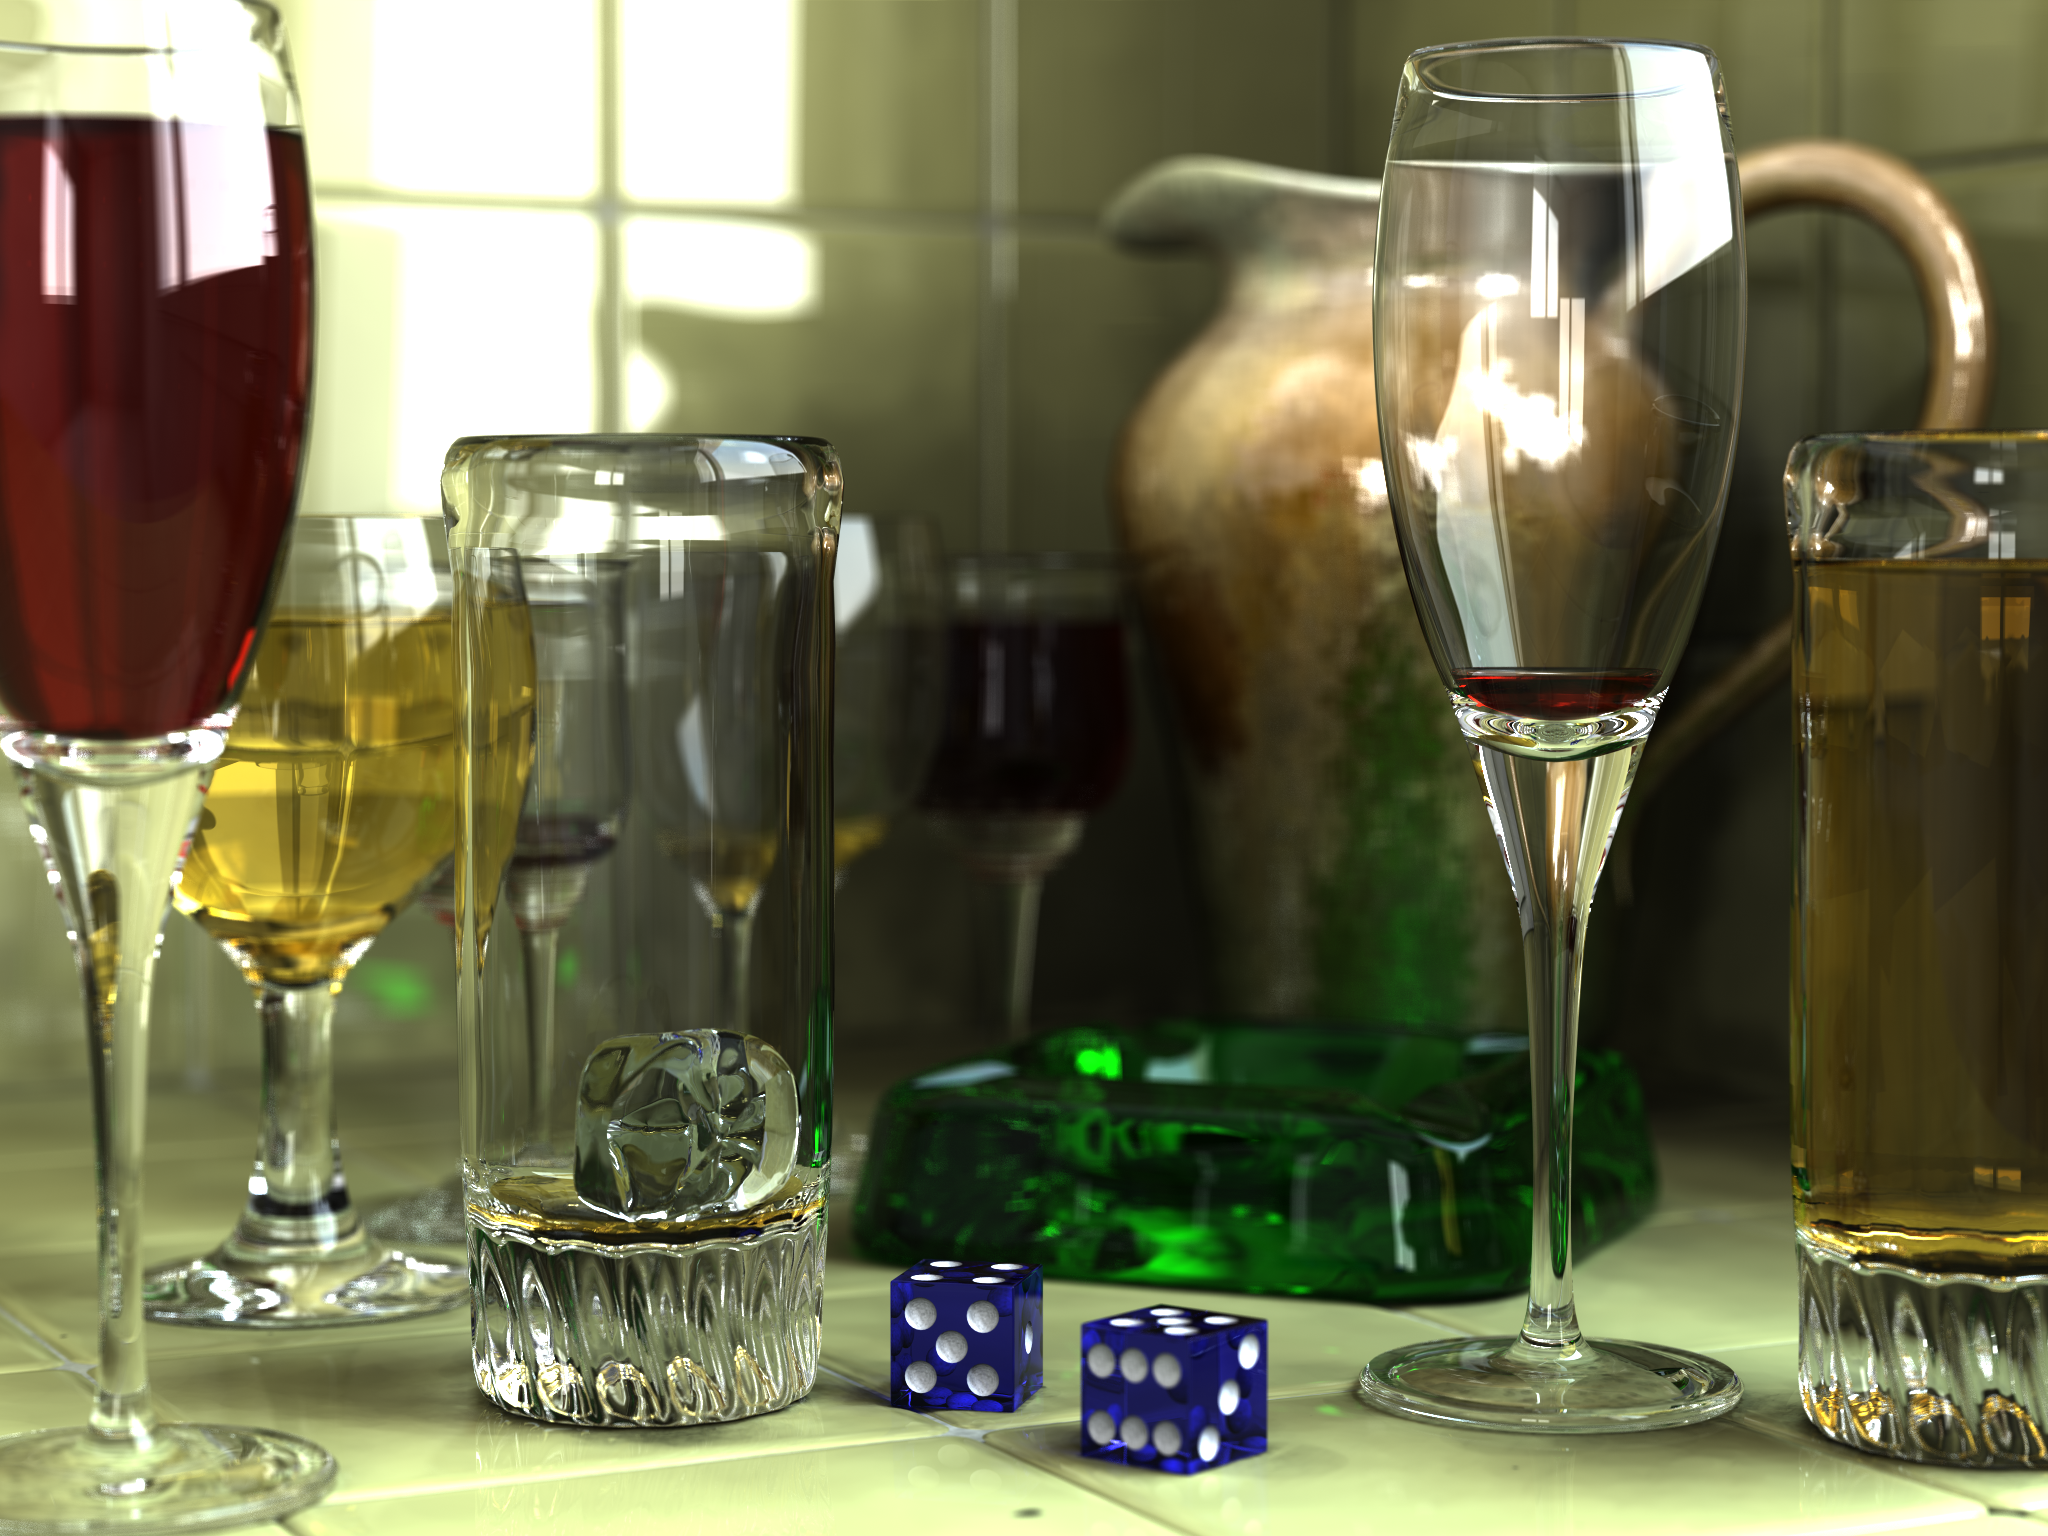
\includegraphics[width=0.5\textwidth]{PhotorealisticRendering}
	\caption{3D modeling systems are often used to produce photorealistic imagery, which is not always the proper best at communicating geometric information as discussed in \cite{JDA08}.
		Notice how difficult it is to discern the edges and faces of the dice,
		how the reflections of the bright light from the window obscure the structure of the glasses, and the shadows make it hard to read the visual extent of the glass hidden in the dark background.
		Image Credit: Gilles Tran on Wikipedia.}
	\label{fig:photorealistic_rendering}
	\end{figure}

	\paragraph{2D Illustration Software.}

	2D illustration software, such as the open source \emph{Inkscape}, are used primarily by designers and communicators to create 2D Scalable Vector Graphics (SVG) illustrations that
	communicate ideas, rather than realistic visual artifacts. They have a lot of capabilities for modifying the colors and stroke sizes of lines and interiors,
	labeling important features with textual boxes and arrows, and compositing different visual objects on top of each other through blending.
	While they are great at manipulating the aesthetics of images, they do not necessarily understand 3D geometry and take it into account in the manipulations
	that they support. Please see Figure: \ref{fig:cornell_box_illustration}, which is an example 2D illustration that we created in \emph{Inkscape} that communicates light transport within a traditional Cornell Box scene.

	\begin{figure}[h]
	\centering
	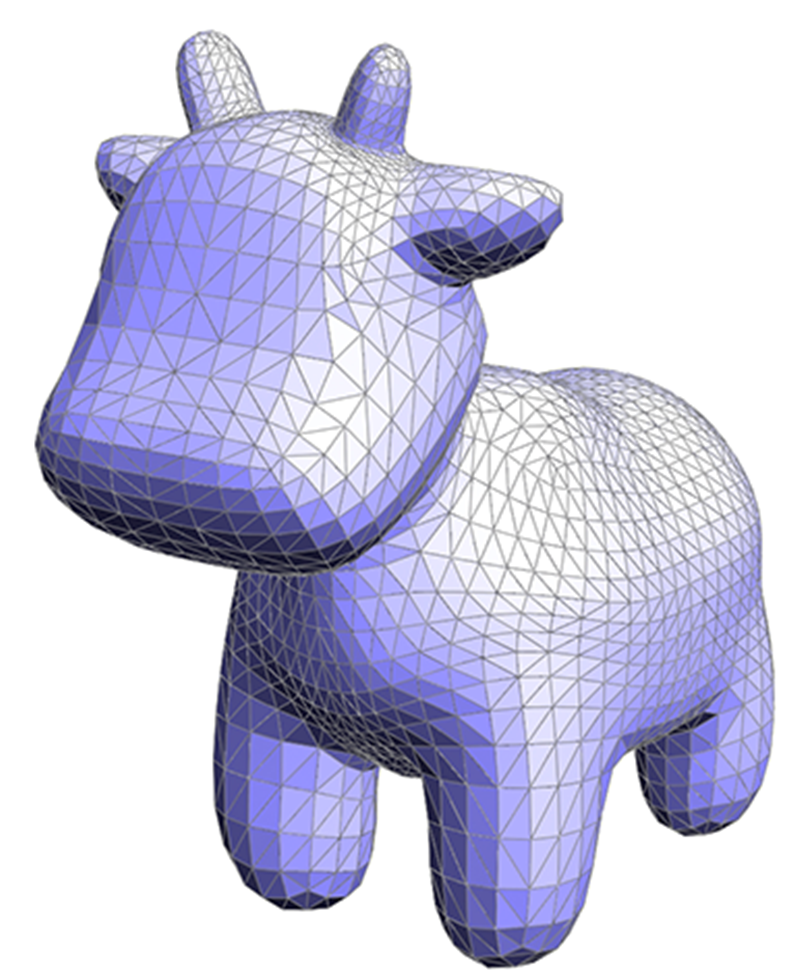
\includegraphics[width=0.3\textwidth]{KeenanCow}
	\caption{A typical 3D model that is manipulated in a 3D modeling program. Note the visual emphasis on representational features associated
			with the discretization of the geometry such as the triangular faces and flat shading, rather than the emphasis on light transport properties emphasized
			in realistic renderings like in Figure: \ref{fig:photorealistic_rendering} or the continuous geometric properties emphasized in our desired system such
			as in Figure: \ref{fig:keenan_style}.}
	\label{fig:keenan_cow}
	\end{figure}

	\paragraph{Geometric Latex.}

	Our goal is to unify these two paradigms to enable the creation of figures that are generated directly from 3D geometric mathematical models 
	and amenable to stylistic modification that takes advantage of the geometric information. In essence, we wish to create a ``geometric \LaTeX" program.
	See Figure: \ref{fig:keenan_style} for an example illustration that
	we could make natively using such a program. We would also be able to easily produce traditional mathematical illustrations such as those found in 
	Tristan Needham's book, \emph{Visual Complex Analysis}. Most high quality mathematical illustrations found in the literature are hand drawn,
	but through our work people should eventually find it easier to create high quality geometric illustrations using software in lieu of non-digital methods.

	\begin{figure}[h]
	\centering
	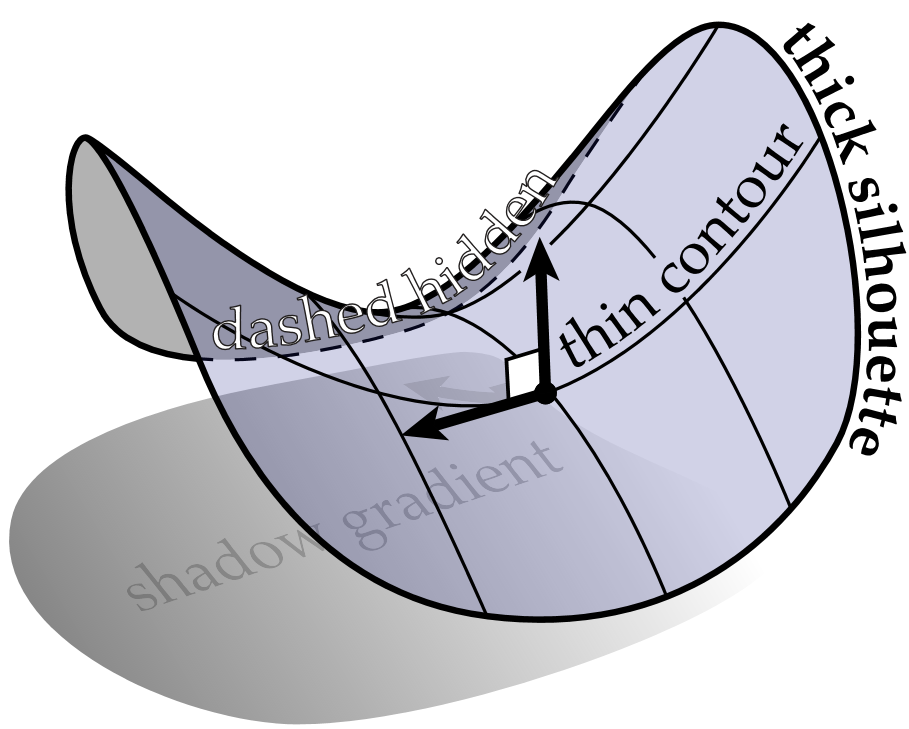
\includegraphics[width=0.5\textwidth]{StylizedFigure}
	\caption{A 3D geometric image created with proper aesthetic design. To create this image, a system would need to model the saddle geometry along
	with its smooth boundary, compute tangents and curvatures,
	extract minimum and maximum curvature curves to defined the local coordinate system, extract smooth silhouette curves, segment curves based on occlusion,
	extract the planar shadow via a silhouette curve projection, and provide user features for curve and tangent aware labels.
	The system would need to be able create gaps at intersections between labels, arrows, and the geometric curves.
	The Image is Courtesy of Keenan Crane.}
	\label{fig:keenan_style}
	\end{figure}

\newpage

	\paragraph{Foundational Problems}
	To realize the goal of a geometric \LaTeX program, we need to solve many problems revolving around the extraction of important curves from 3D models
	such as those used for stylization in Figure \ref{fig:keenan_style}. In general, we need to develop algorithms for extracting representations for any curves
	that communicate important visual or geometric information or that may be required for the conversion between the processes defined within each paradigm
	that are not yet compatible with each other, such as fills in 2D and shadow casting in 3D. In particular, we have investigated the extraction of silhouette curves and parameter curves,
	as well as critical points and integral curves for the Morse-Smale complex. We have also investigated various sub problems for curve extraction,
	including locating \emph{every} curve, finding unique representative points for every curve, gradient descent methods, and planar curve projections.

\newpage

\section{Background/Prior Work}

	\subsection{Important 2D curves for projected 3D models.}

		Various curves on surfaces communicate important geometric information. Here is a list of some relevant curves that folks have
		tried to extract from surfaces in the past.

\begin{itemize}
	\item 	\textbf{Parameter curves} are useful in showing lines along a collection of quadrilaterals and showing global coordinate systems.
			They are useful primarily because 3D models are often created using a discretization that follows the symmetries and geometric structure
			of the object they are modelling.
	\item 	\textbf{Silhouette curves} communicate the visual extent of the model and the boundary.
			The projection of silhouette curves onto a plane determine the shadows that a surface casts.
			The collection of silhouette curves for a surface without double negative curvature defined with regards to every viewing direction constrained to a plane
			is sufficient to describe the geometry of the surface.
	\item 	\textbf{Minimum - Maximum curvature curves} communicate the curvature of the model and locally intuitive coordinate systems.
	\item        \textbf{Geodesic curves} communicate the path on the surface of minimum distance between two points on a surface.
	\item 	\textbf{Integral Lines}: lines that follow the gradient of a function defined on a surface from one critical point to another. These may be used to form the Morse-Smale complex
			which segments the model into regions with similar monotonic functional behavior.
\end{itemize}

	\subsection{Prior Extraction Methods}

	\paragraph{2D Curve Extraction Methods.}

		Many people have extracted silhouette curves by simply tracing the exterior boundary of a 2D rasterization of the surface. This approach suffers from 
		discretization and sampling problems and does not provide much information about the 3D geometric structure of the silhouette curves.
		For instance, they can't be used to compute direct shadows.
		It also may be possible to extract silhouette curves using an algorithm akin to the marching squares, but again it would suffer from the same sorts of problems.
	
	\paragraph{3D Curve Extraction Methods.}

	Stroila et. al. were able to extract silhouette, shadow, gleam, and other curves via particle systems. They have also studied practical ways to utilize these curves
	for illustration by describing how to sort, orient, identify, and fill them as closed regions. \cite{SEH08}
	Their methods mainly rely on the intersections of implicit surfaces and produce high quality curves, but it would be difficult and computationally
	inefficient to fit a particle system to complicated arbitrarily defined surfaces, such as Catmull-Clark subdivision surfaces.
	
	\subsection{Catmull-Clark Subdivision Surfaces}

		Catmull-Clark subdivison surfaces are a very popular subdivision method for quadrilateral meshes, that produces $\mathcal{C}^{1}$
		limit surfaces (i.e. surfaces with continuous positions and tangents) that approximate points that lie along meshes of arbitrary topology. \cite{Catmull98}
		The stencils that define this subdivision scheme are shown in Figure: \ref{fig:Catmull-Clark-stencils} and Figure: \ref{fig:Catmull-Clark}
		shows an example series of Catmull-Clark subdivision steps on a cube control mesh with a sphere like limit surface.

		\begin{figure}[h]
		\centering
		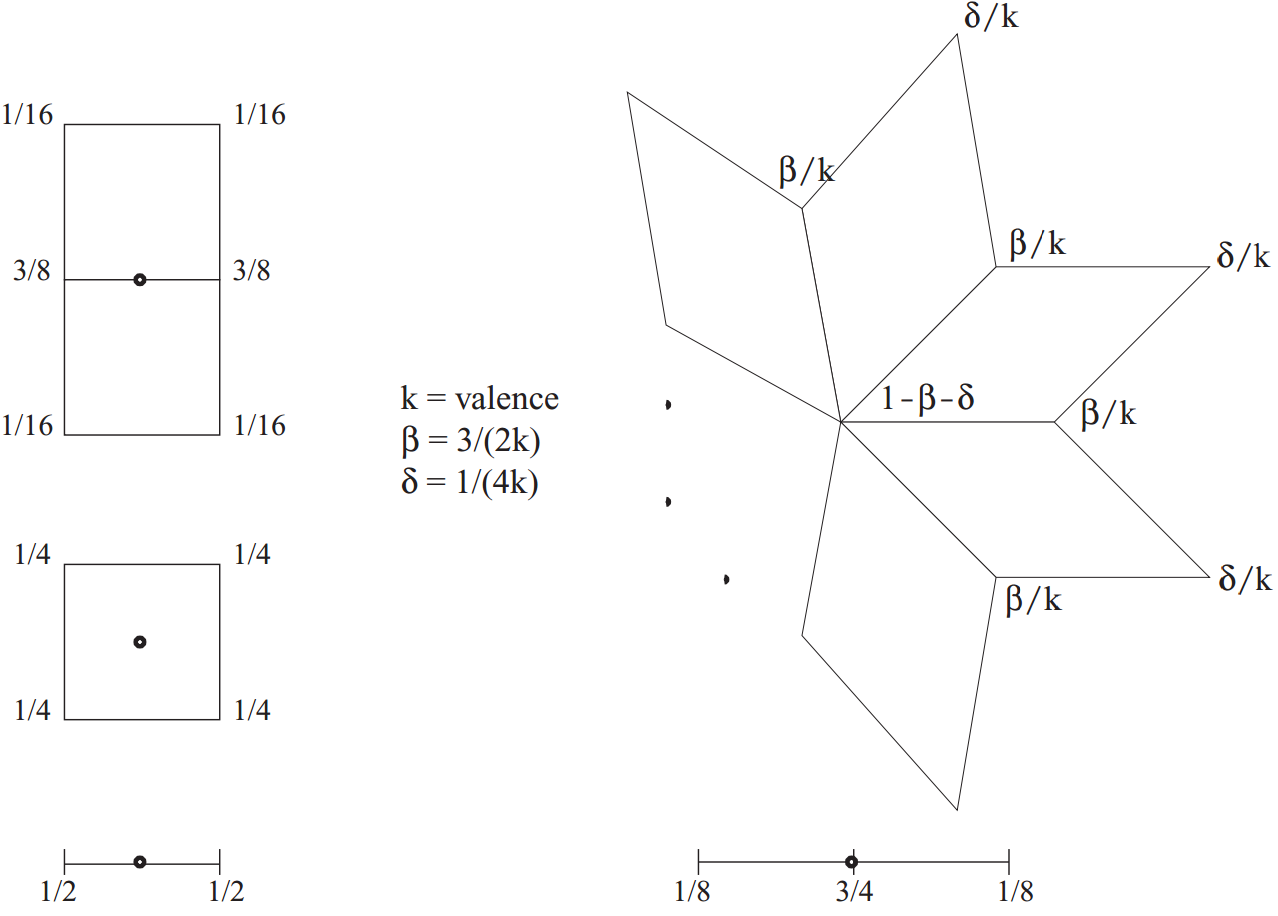
\includegraphics[width=0.75\textwidth]{Catmull_Clark_stencils}
		\caption{The standard stencils for a Catmull-Clark subdivision step are shown that specify the linear combinations used to 
				compute the new edge points, face points, and vertex locations. The stencils at the bottom of the figure show the stencils 
				for boundary edge points and vertex locations. Image Credit: \cite{BS}.}

		\label{fig:Catmull-Clark-stencils}
		\end{figure}

		\begin{figure}[h]
		\centering
		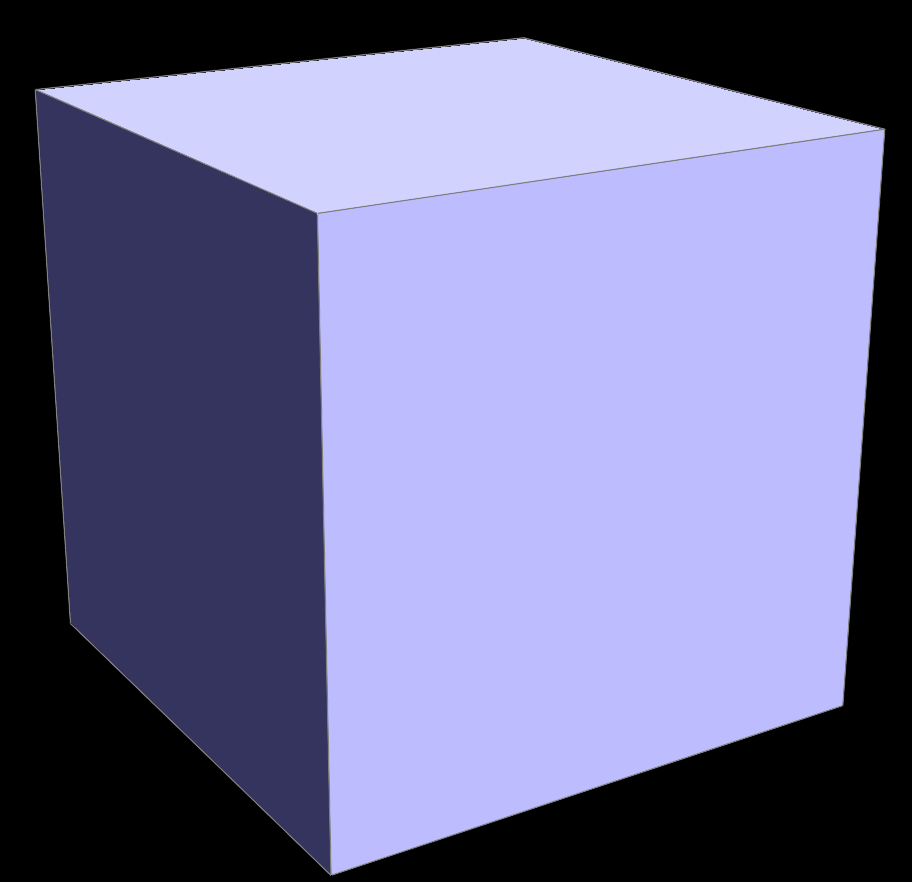
\includegraphics[width=0.3\textwidth]{cc0}
		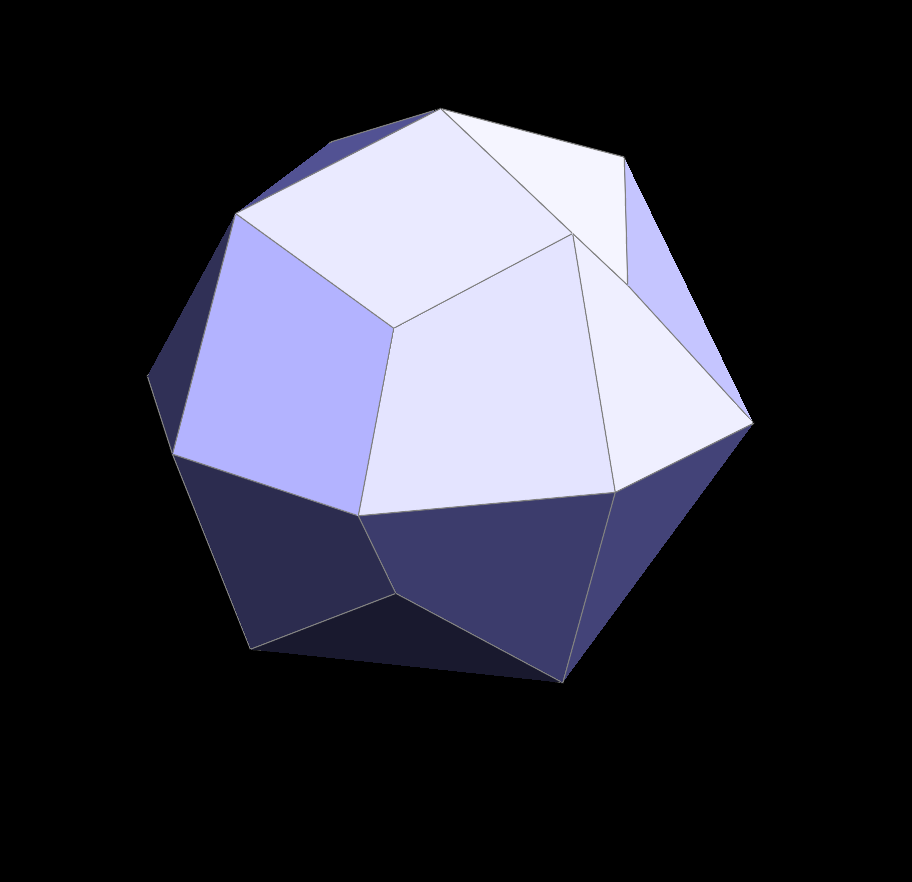
\includegraphics[width=0.3\textwidth]{cc1}
		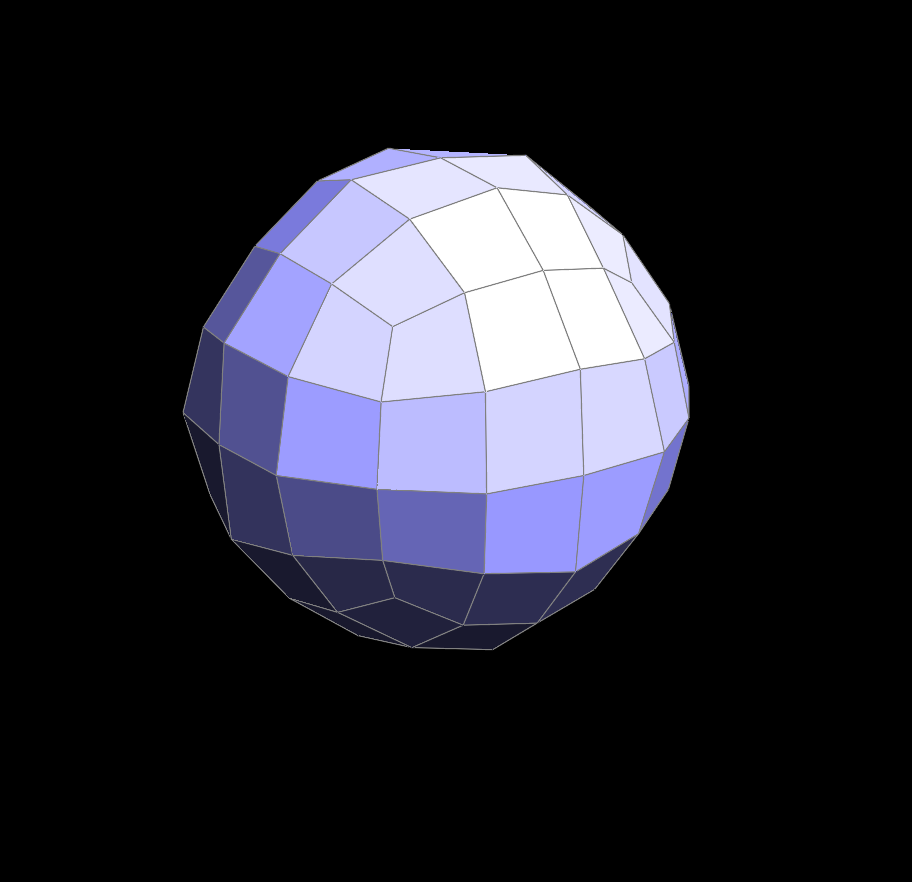
\includegraphics[width=0.3\textwidth]{cc2}
		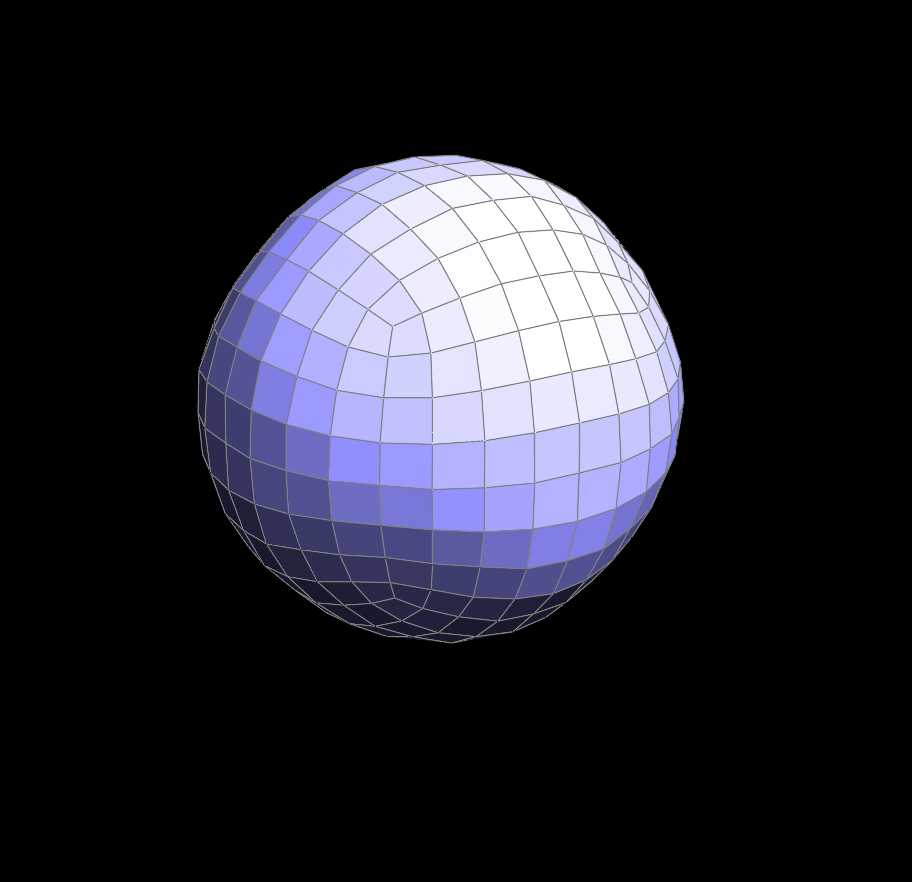
\includegraphics[width=0.3\textwidth]{cc3}
		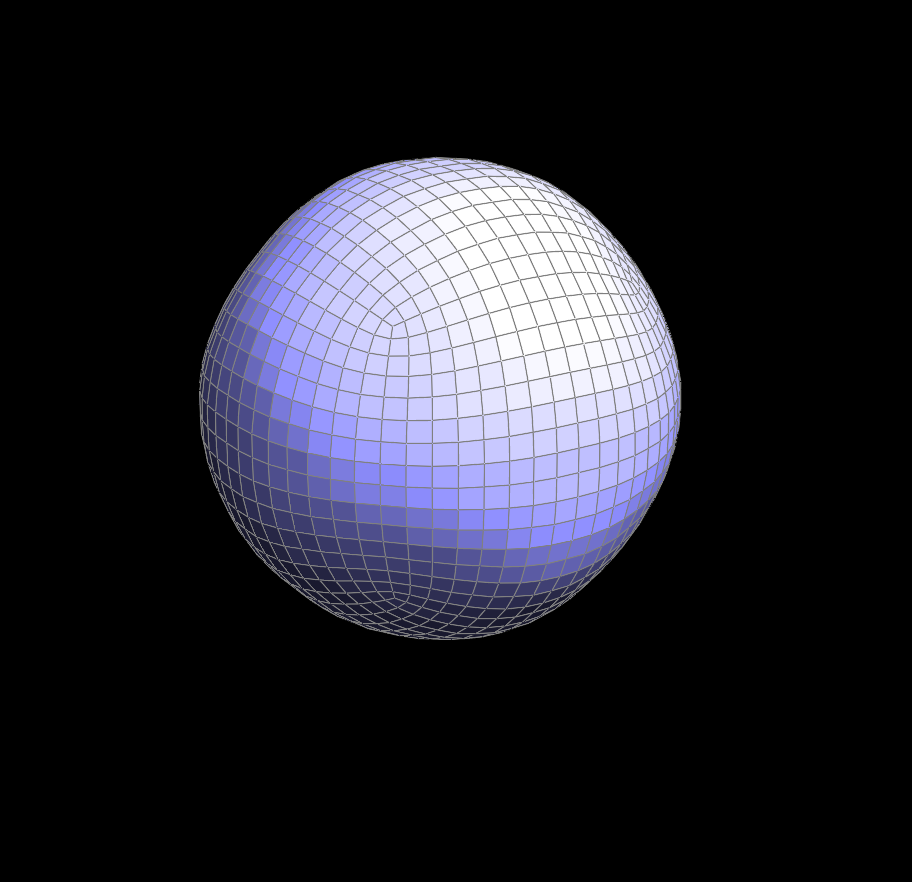
\includegraphics[width=0.3\textwidth]{cc4}
		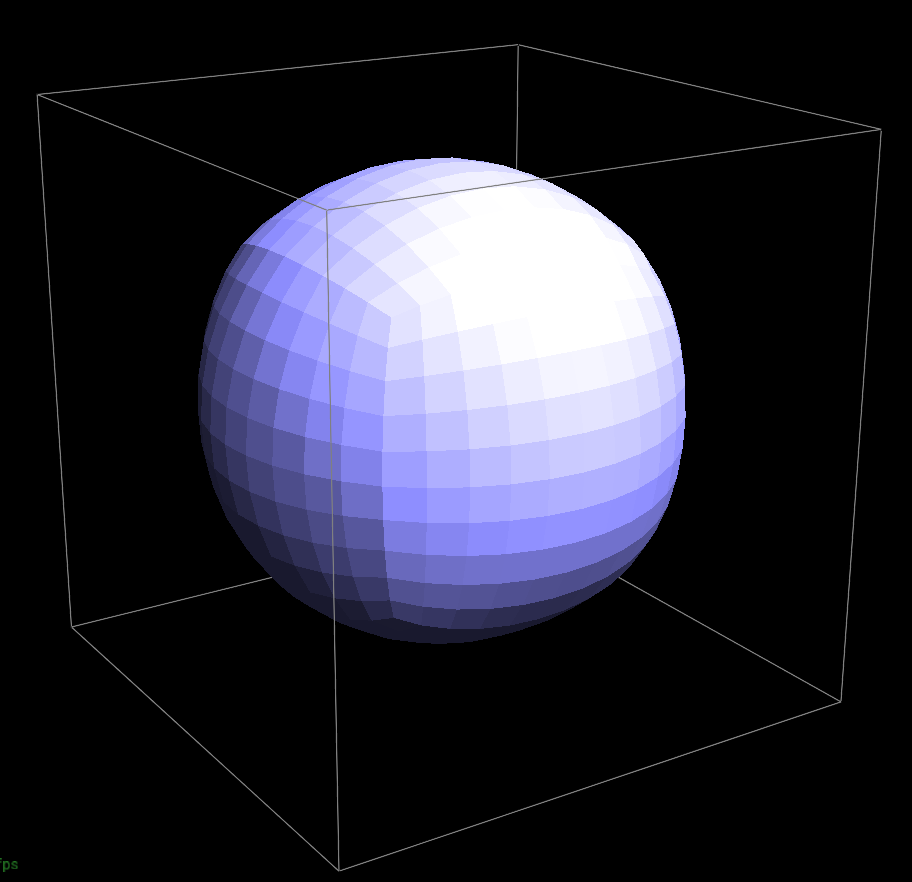
\includegraphics[width=0.3\textwidth]{cc_loop_shaeffer}
		\caption{A cube mesh is shown along with 4 subdivision steps using the Catmull-Clark subdivision algorithm. The steps proceed from left to right, top to bottom.
				The bottom right figure shows the Loop-Schaefer geometry patch approximation of the Catmull-Clark limit surface.}
		\label{fig:Catmull-Clark}
		\end{figure}

		\paragraph{Prior Linear Patch Methods}
		Naively we could directly evaluate curves over the linear patches defined on standard polyhedral 3D models,
		but much like the results found in \cite{Eisemann08},
		such lines would jitter back and forth over boundaries and would not converge to smooth natural and correct looking curves even after 
		substantial subdivision of the surface. See Figure \ref{fig:Eisemann_linear_patches} for example of Eisemann et Al's attempt to extract silhouette
		curves from linear patches. We therefore wish to work on Catmull-Clark Subdivision surfaces that allow us to take a discrete quadrilateral control mesh
		and perform calculations on its continuous limit defined subdivision surface, instead of any intermediate discrete representation.
		See Figure : \ref{fig:subDDef} for an illustration of control meshes and limit surfaces.

		\begin{figure}[h]
		\centering
		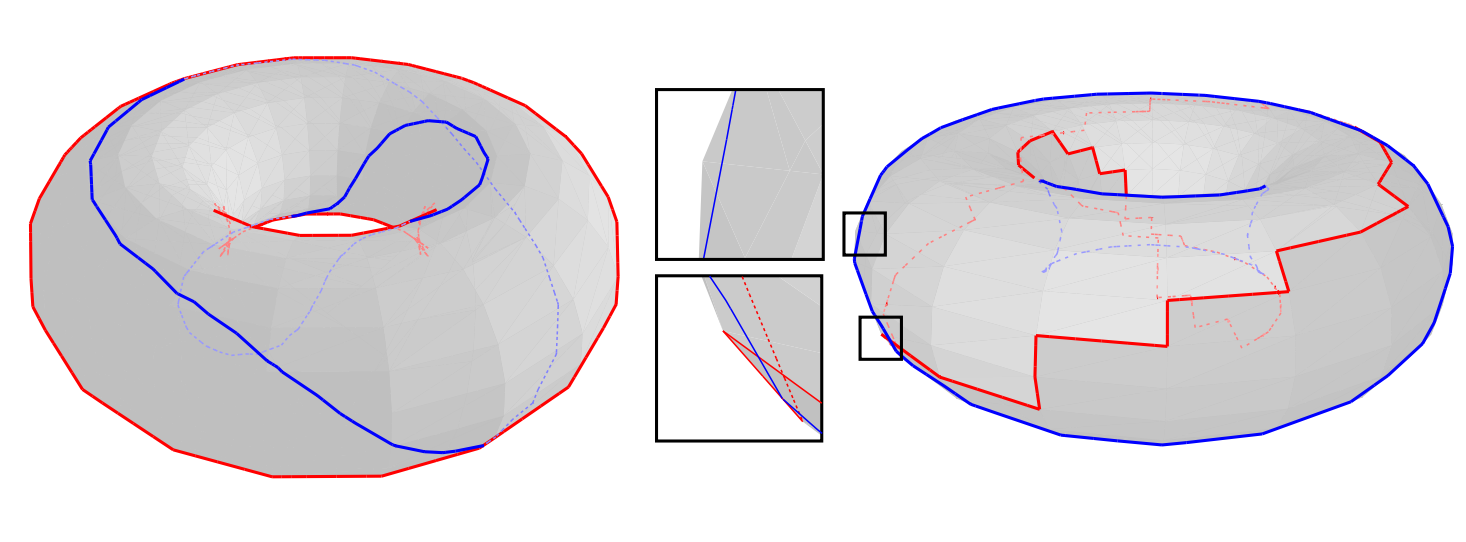
\includegraphics[width=0.5\textwidth]{Eisemann08_linear_patches}
		\caption{Linear Patches Silhouette curves either produce staircase patterns or don't properly lie on the geometry, even in the limit. Image Credit: \cite{Eisemann08}.}
		\label{fig:Eisemann_linear_patches}
		\end{figure}

		\begin{figure}[h]
		\centering
		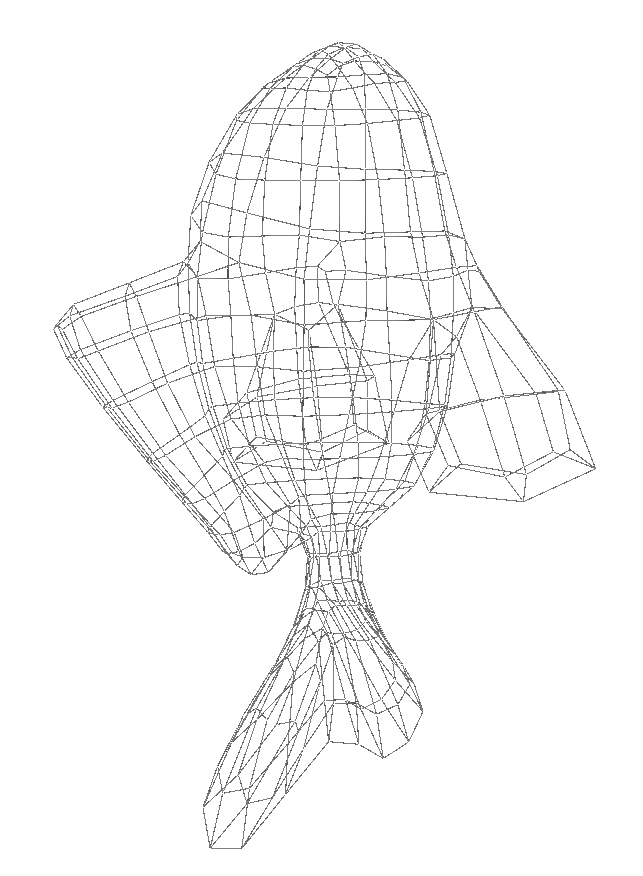
\includegraphics[width=0.3\textwidth]{fish_cm}
		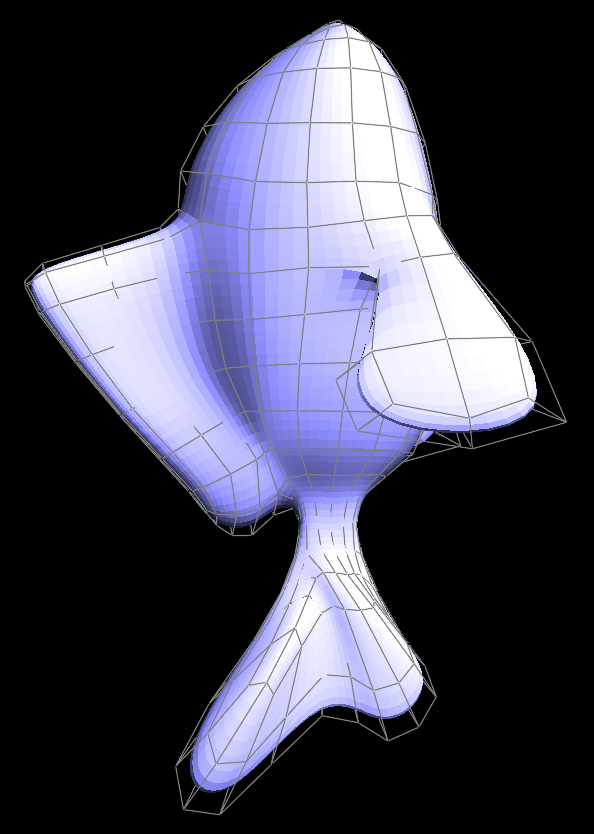
\includegraphics[width=0.3\textwidth]{fish_cm_and_patch}
		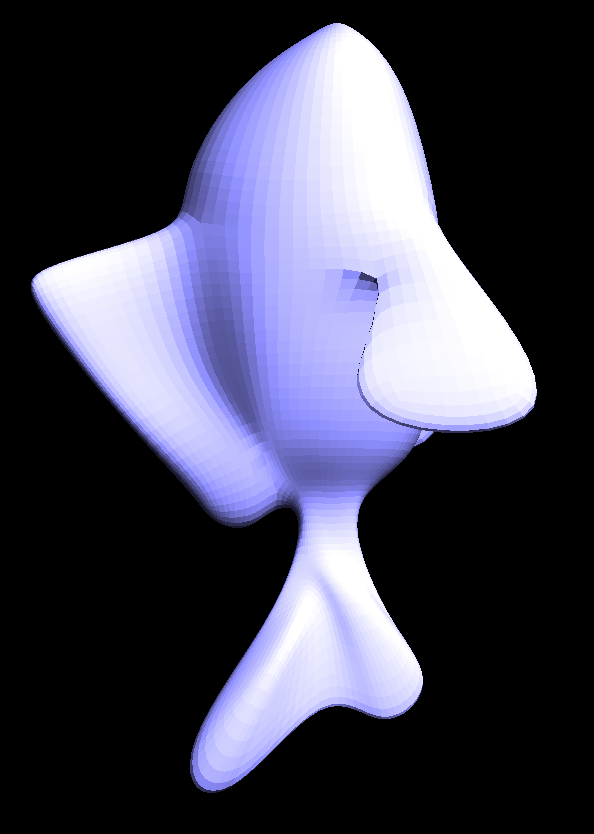
\includegraphics[width=0.3\textwidth]{fish_patch}
		\caption{A model of a fish represented from on the left by its control mesh and on the right by a geometry patch approximation of its Catmull-Clark limit surface.}
		\label{fig:subDDef}
		\end{figure}

	\paragraph{Finite Element Methods}

		There has been work with finite element methods and Catmull-Clark, such as those using quadratic interpolants discussed in \cite{Zorin06} and \cite{PXXZ15}.
		We have avoided finite element methods in our computation of positions, tangents and curvature, because the surfaces we will be using as discussed in the next section
		make it very easy to analytically evaluate and differentiate the surface position functions.


	\subsection{Loop-Shaeffer Approximations}

		No matter how finely we refine a traditional Catmull-Clark surface, it will still be a collection of linear patches which suffer from the same problems as
		in \cite{Eisemann08}. Jos Stam came up with a method of directly evaluating Catmull-Clark limit surfaces at arbitrary parameter values\cite{Stam98},
		but it is based on matrix diagonalization methods and would difficult and less efficient to use in the extraction algorithms we are interested in.
		
		We get around these problems by directly computing a continuous and differentiable approximation of the limit surface
		via the scheme described in \cite{Loop}
		We can create a one-to-one correspondence between faces in the control mesh and bicubic Bezier surfaces (a.k.a. ``patches") that approximate the 
		limit Catmull-Clark subdivision surface that the faces represent. See Figure: \ref{fig:Catmull-Clark} for an illustration of how the Loop-Schaeffer is
		a high quality approximation for a limit Catmull-Clark surface.
		
		\begin{figure}[h]
		\centering
		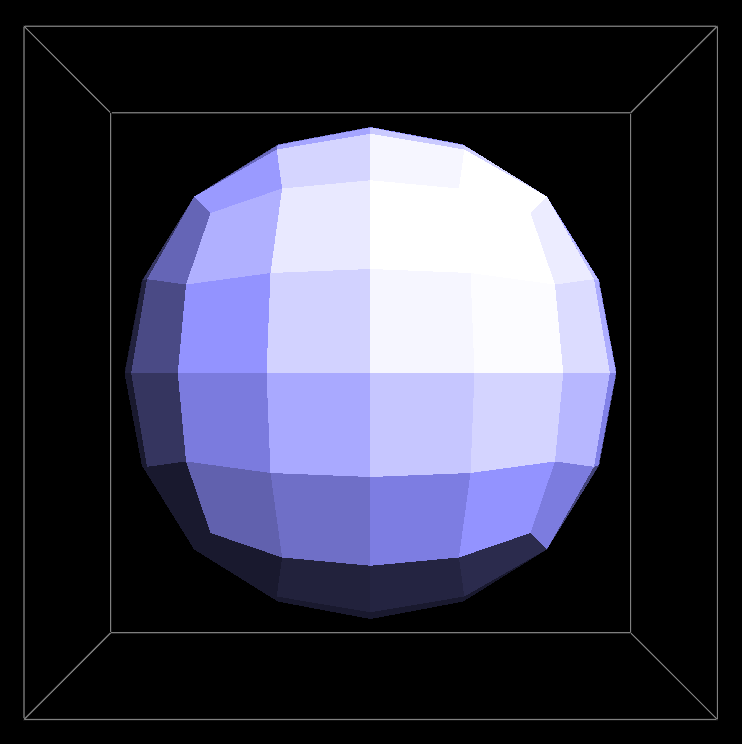
\includegraphics[width=0.3\textwidth]{cube_0p}
		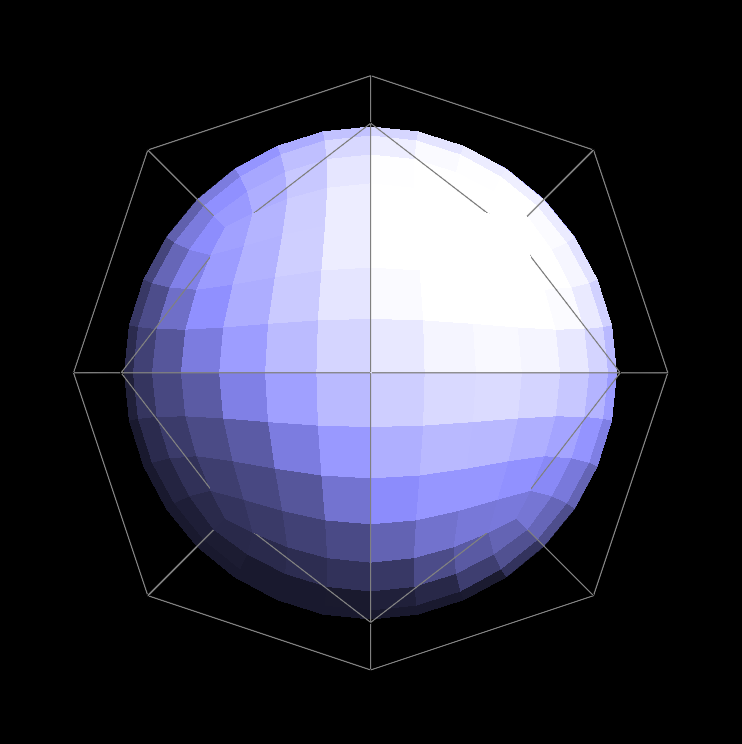
\includegraphics[width=0.3\textwidth]{cube_1p}
		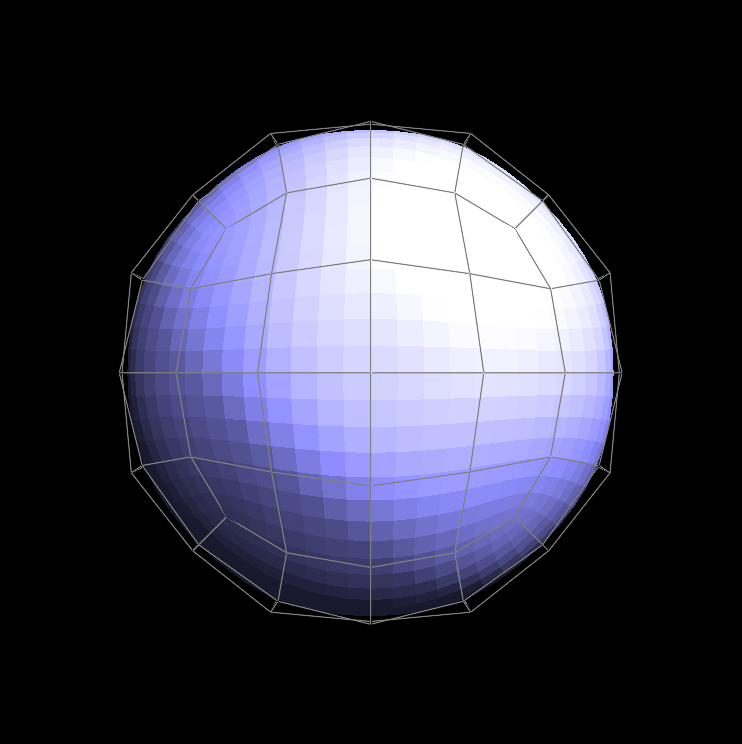
\includegraphics[width=0.3\textwidth]{cube_2p}
		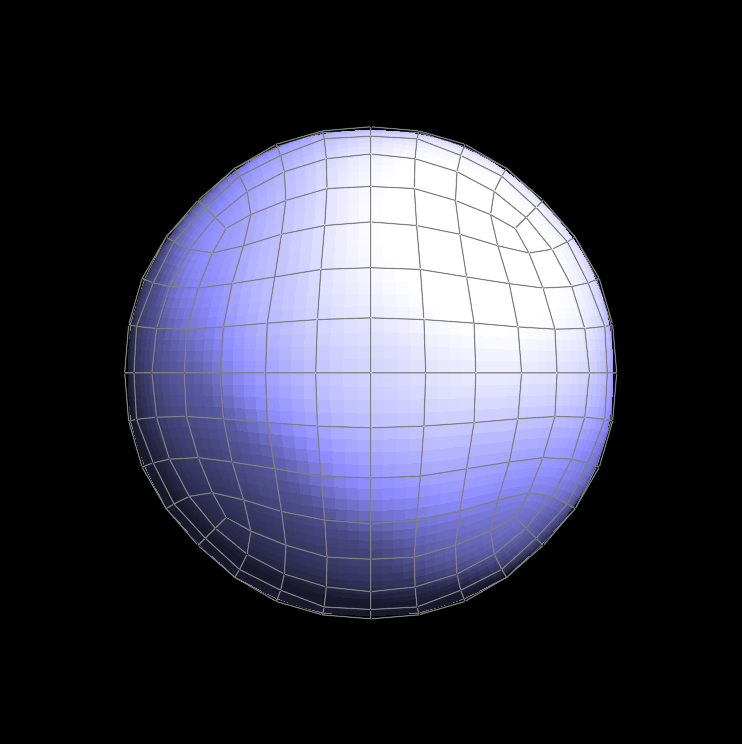
\includegraphics[width=0.45\textwidth]{cube_3p}
		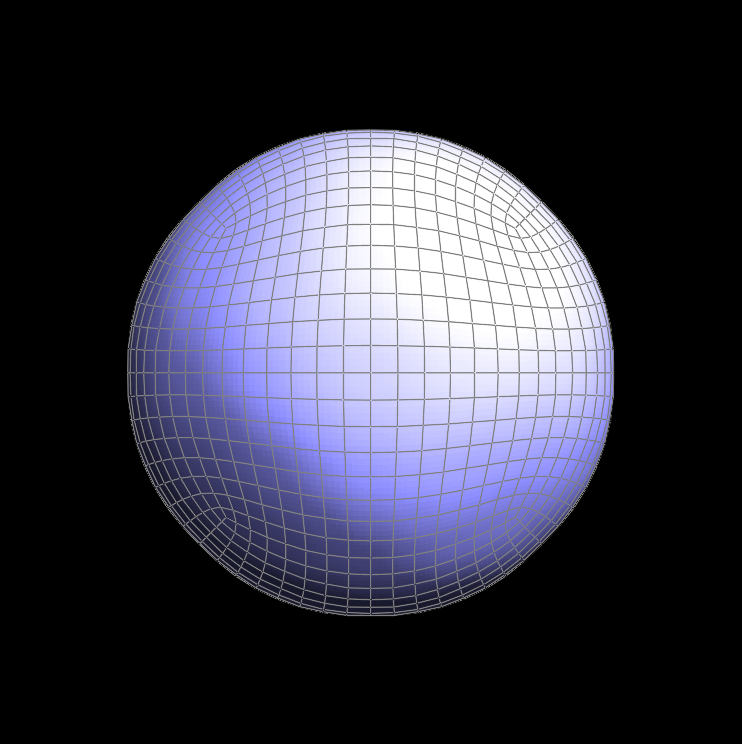
\includegraphics[width=0.45\textwidth]{cube_4p}

		\caption{A Loop-Shaeffer geometry patch surface is shown along with a successively refined Catmul-Clark control mesh which converges to
		a limite surface that is very similar to the bicubic patch approximation.}
		\label{fig:Catmull-Clark}
		\end{figure}

		We then able to derive control points for a geometry patch which we will denote $G_{ij}$ (Figure: \ref{fig:G}) and two tangent patches,
		denoted $U_{ij}$ and $V_{ij}$ (Figure: \ref{fig:dUdV}), one for each principal parameter direction along the bicubic patch.
		The tangent patches are necessary, because the geometry patches only exhibit G0 continuity in the presence of extraordinary vertices (i.e. 
		vertices with degree other than 4.)
		This means that the neighboring geometry patch boundaries having matching positions, but different tangent vectors.
		Since any quadrilateral mesh that is not homeomorphic to a torus must contain an extraordinary vertex,
		it is essential that we use the tangent patches to ensure effective differentiability everywhere along the surface formed by the union of the bicubic patches.
		
		For the remainder of the paper, we will be referring to these Loop - Schaefer Geometry and Tangent patch defined surfaces defined on quadrilateral meshes
		whenever we use the term ``surface". We will assume that these surfaces do not contain boundaries.

		\begin{figure}[h]
		\centering
		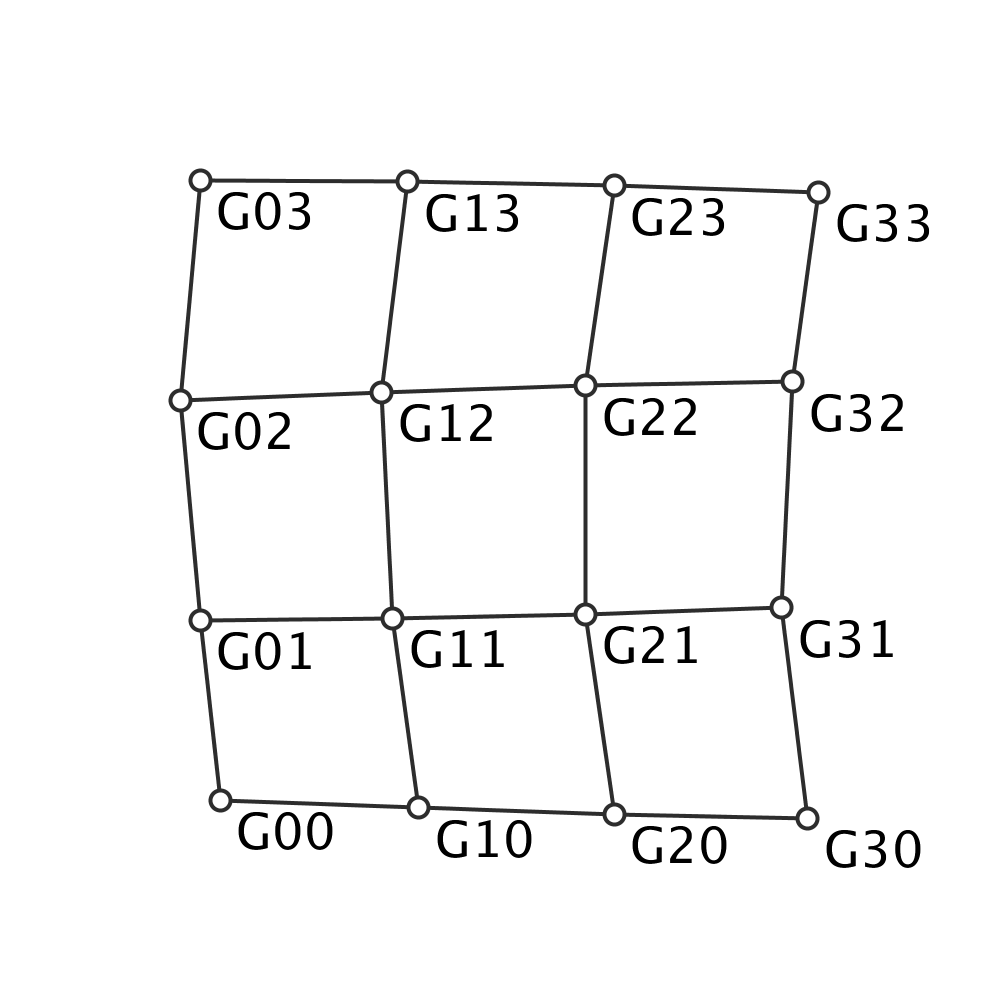
\includegraphics[width=0.35\textwidth]{GeometryPatchControlPoints}
		\caption{Geometry Patch Control Points for a single control mesh face.}
		\label{fig:G}
		\end{figure}

		\begin{figure}[h]
		\centering
		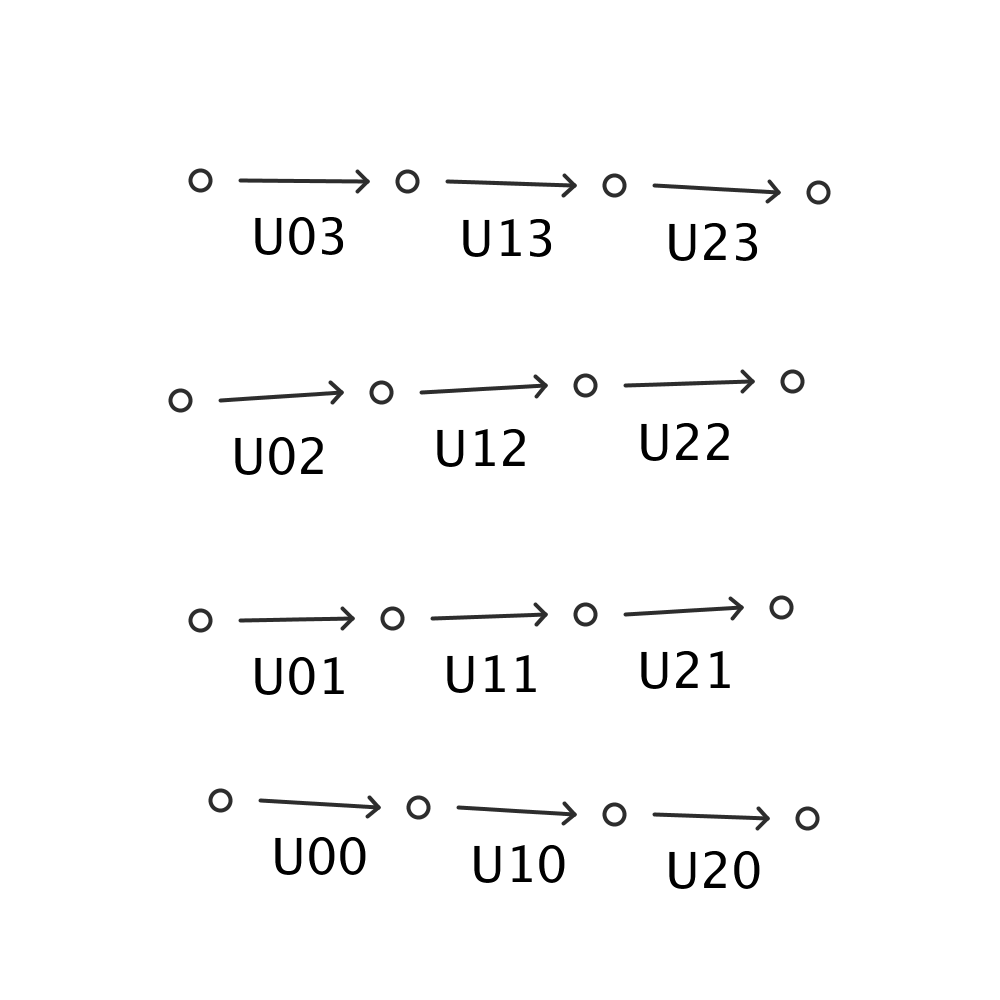
\includegraphics[width=0.35\textwidth]{duPatch}
		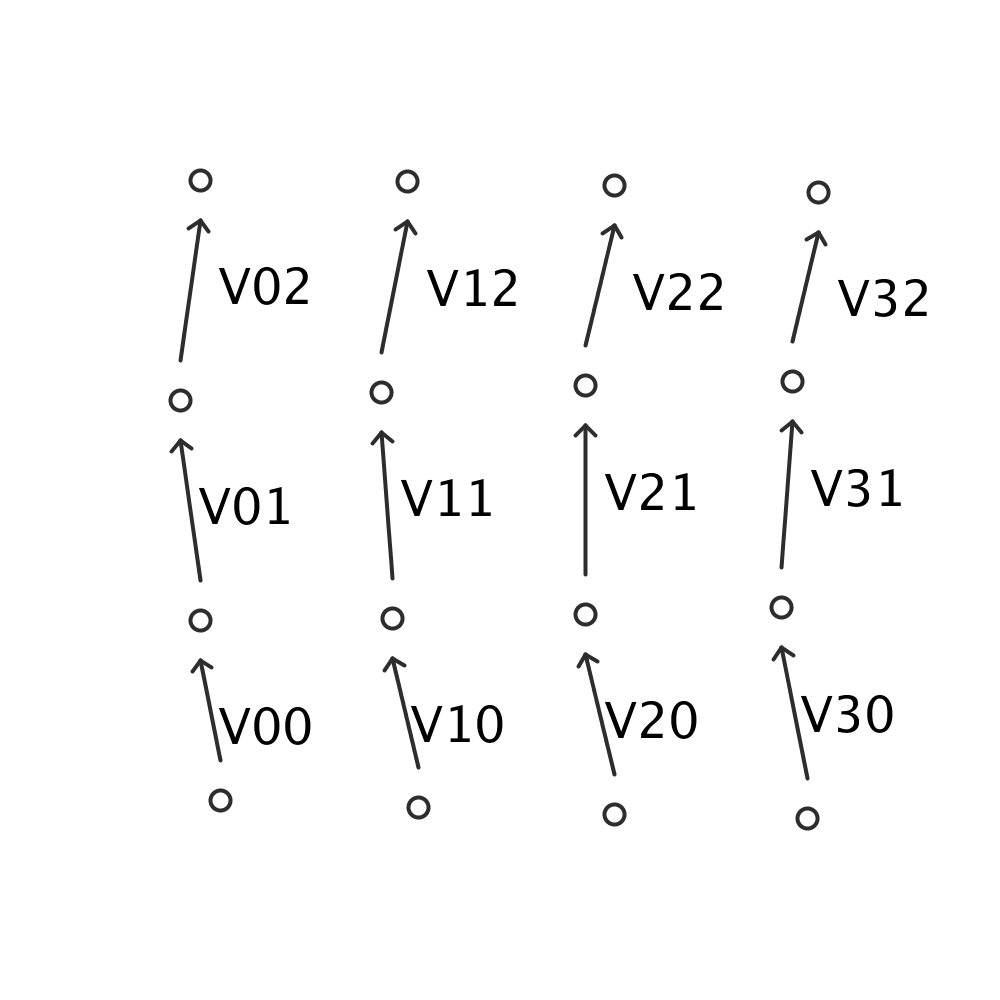
\includegraphics[width=0.35\textwidth]{dvPatch}
		\caption{$\partial u$ and $\partial v$ tangent patch control vectors for a single control mesh face.}
		\label{fig:dUdV}
		\end{figure}

\newpage

\section{Methodology}

	\subsection{Definitions and Calculus on Bicubic Patches}
	
	In this section we will discuss some fundamental calculus computations involving the patches that will be used in curve extraction algorithms.

		\paragraph{Bezier Surfaces}
		A \emph{bicubic patch} is a \emph{Bezier surface} that can be represented explicitly in terms of the so-called
		\emph{Bernstein polynomials}, and interpolates data points.
		The beauty of the bicubic patch approximations for Catmull-Clark subdivision surfaces described by Loop and Schaefer
		is that they allow us to transition from discrete math to well defined continuous math.

		The \emph{Bernstein polynomials} are defined as follows:

		$$\mathcal{B}_{i, n}(x) = \mathcal{B}_{i}^{n}(x) = \binom{n}{i}x^{i}(1-x)^{n-i} \; \textbf{for} \; i \in \{0, \cdots, n\}  $$
		
		Two-dimensional \emph{Bezier surfaces} are defined parametrically as follows: 
		
		$$[0, 1] \times [0, 1] \rightarrow \mathbb{R}^{3} : \sum_{i=0}^{n}{\sum_{j=0}^{m}{\mathcal{B}_{i}^{n}(u) \mathcal{B}_{j}^{m}(v) C_{i, j}}}$$
		
		where $n, m$ is the degree of the surface, which is represented by $(n + 1) \cdot (m + 1)$ control points denoted generically here by $C_{ij}$.
		
		\paragraph{Geometry Patches}

		The geometry patch surfaces are of degree (3, 3) and are therefore represented by the 16 control points $G_{ij}$ as follows:
		
		$$g(u, v) = \sum_{i=0}^{3}{\sum_{j=0}^{3}{\mathcal{B}_{i}^{3}(u) \mathcal{B}_{j}^{3}(v) G_{i, j}}}$$
		
		\paragraph{Partials Defined by Geometry Patches}

		We can easily take partial derivatives of a Geometry Patch as follows:

		$$g_{u^{m}v^{n}} = \frac{\partial g}{\partial u^{m} \partial v^{n}} = \sum_{i=0}^{3}{\sum_{j=0}^{2}{\mathcal{B}_{i, 3}^{(m)}(u) \mathcal{B}_{j, 3}^{(n)}(v) G_{i, j}}}$$

		where $m$ and $n$ are the degrees of differentiation in $u$ and $v$ respectively.

		\newpage

		\paragraph{Partials Defined by Tangent Patches}
		
		We can easily take partials of $g$ in $u$ and $v$ by differentiating the relevant $u$ or $v$ parameterized Bezier function,
		but for the most part we will not make use of this pleasantry, because the geometry patches may be non-differentiable on the boundaries.
		We will instead evaluate the partials from the tangent patches.
		
		\begin{equation} \label{eq:g_u}
		g_{u} := \frac{\partial g}{\partial u} = \sum_{i=0}^{3}{\sum_{j=0}^{2}{\mathcal{B}_{i}^{3}(u) \mathcal{B}_{j}^{2}(v) U_{i, j}}}
		\end{equation}

		\begin{equation} \label{eq:g_v}
		g_{v} := \frac{\partial g}{\partial v} = \sum_{i=0}^{2}{\sum_{j=0}^{3}{\mathcal{B}_{i}^{2}(u) \mathcal{B}_{j}^{3}(v) V_{i, j}}}
		\end{equation}

		\paragraph{Normals}

		The normal direction is defined for any point on the surfaces as follows:

		$$N(u,v) = g_{u} \times g_{v} (u, v)$$

		Typically normal vectors would be normalized to a unit length, but for the purpose of extracting silhouette curves
		this normalization will not affect the final results, which enables us to use the simplified (unnormalized) expression.
		Not only is the simplified expression easier to differentiate symbolically, it also outputs 3 dimensional vectors containing multinomials,
		which work well with the root finding algorithms in Section : \ref{section:rootFindingGeometryPatch}.
		
		\subsubsection{Gradient Descent}
		\label{section:GD}

		Many of our algorithms rely on gradient descent to optimize various functions on surfaces. A proper selection of step sizes is important for these
		operations. If the steps are too small, then performance will suffer due to slow convergence. If the steps are too large, then the optimization procedure may overshoot local minima and fail to converge.
		Gradient descent may be performed on any function $f : \mathbb{R}^{n} \rightarrow \mathbb{R}$ :  provided that $f$ is differentiable.
		A direction $u \in \mathbb{R}^{n}$ is a \emph{search direction} if the directional derivative of $f$ along $u$ is negative.
		In other words for a search direction $u$, the following holds:

		$$ D_{u}f = \nabla f \cdot u < 0$$

		Given an initial point $x_{0}$ and a search direction $u$, we search for a new point $x_{1} := x_{0} + \tau u$ that is of a step size that is guaranteed to make progress towards finding a local minima. 
		The step size should therefore satisfy two conditions as follows:

		\begin{enumerate}
		\item The \textbf{Armijo condition} $f(x_{0} + \tau u) \le f(x_{0}) + c_{1} \tau D_{u} f(x_{0})$\\
		\item The \textbf{Wolfe condition} $|D_{u}f(x_{0} + \tau u)| \le c_{2}|D_{u}f(x_{0})|.$
		\end{enumerate}

		where $c_{1}, c_{2} \in \mathbb{R}$ are any two constants such that $$0 < c_{1} < c_{2} < 1.$$

		We can then compute the step size via Algorithm: \ref{alg:step_size}.

		\begin{algorithm}
		\caption{Given an initial point $x_{0}$ and a search direction $u$, this algorithm searches for a point that fulfills the \textbf{Armijo} and \textbf{Wolfe} conditions makes progress towards finding a local
				minimum. Please refer to \ref{section:GD}.}
		\label{alg:step_size}
		\begin{algorithmic}
			\STATE \textbf{begin}
			\STATE $\alpha \leftarrow 0$
			\STATE $\beta \leftarrow +\infty$
			\STATE $\tau \leftarrow 1$
			\REPEAT
				\IF{Armijo is not satisfied}
					\STATE $\beta \leftarrow \tau.$
				\ELSIF{Wolfe is not satisfied}
					\STATE $\alpha \leftarrow \tau$
				\ELSE 
					\STATE BREAK.
				\ENDIF
				\IF{ $\beta < +\infty$}
					\STATE $\tau \leftarrow (\alpha + \beta)/2$
				\ELSE
					\STATE $\tau \leftarrow 2 \alpha$
				\ENDIF
			\UNTIL{BREAK}
			\STATE \textbf{end}

		\end{algorithmic}
		\end{algorithm}

		For the purposes of this thesis, we will label gradient descent operations as follows:
		$$ x_{1} = \text{GD}(f, x_{0})$$ where $x_{0}$ is the initial point, $f$ is a differentiable function, and $x_{1}$ is the resultant minimization of the function.
		
		\newpage
		\subsubsection{The Visibility Function}

		In the context of this thesis, we will define the \emph{visibility function} as a measure of
		whether the surface is forward or backward facing relative a viewing direction. This is not to be confused with occlusion, which is a measure of
		how many surfaces obscure a surface point from a viewer.
		Given a fixed yet arbitrary viewing direction $E$ we can define the \emph{visibility function} as follows:

		$$f(u, v) = N(u, v) \cdot E$$

		A location $(u, v)$ in parameter space on a surface is visible if and only if $f(u, v)$ is negative.
		Note that the location may still be occluded by another portion of the geometry.
		Also note that we are assuming an orthonormal viewing direction, instead of a perspective projection,
		because it simplifies our mathematics. \cite{XJY98}

		\paragraph{Silhouette Curves and Points}

		A Silhouette point $p$ is any point such that the visibility function is zero. In other words the following must hold:
		$$p = g(u, v) \textbf{ and } f(u, v) = 0$$

		A silhouette curve contains a closed ordered set of silhouette points. In other words they are defined as the boundary between the visible and non-visible regions of the surface.

		\paragraph{Behavior of Visibility Function}

			Assuming that the viewing direction $E$ has unit length, the following properties hold for the visibility function $f$:

			\begin{itemize}
			\item $f$ has a bounded range as follows: $-|N| \le f(u, v) \le |N|$
			\item $f$ has a Global Minimum when $f(u, v) = -|N|$.
			\item $f$ has a Global Maximum when $f(u, v) = |N|$.
			\item Silhouette curves are defined when $f(u, v) = 0$.
			\item The \emph{front side} of a surface is defined by $f(u, v) < 0$
			\item The \emph{back side} of a surface is defined by $f(u, v) < 0$
			\end{itemize}

		\newpage
		\paragraph{Partials of the Visibility Function}

			The first order partial derivatives for the visibility function may be derived as follows using applications of the product rule for derivatives of cross products:

			\begin{align*}
			N(u, v) &= g_{u} \times g_{v} (u, v)\\
			f  &= E \cdot (P_{u} \times P_{v})\\
			\frac{\partial f}{\partial u} = f_{u} &= E \cdot (g_{u^{2}} \times g_{v} + g_{u} \times g_{uv})\\
			\frac{\partial f}{\partial u} = f_{v} &= E \cdot (g_{uv} \times g_{v} + g_{u} \times g_{v^{2}})\\
			\end{align*}

			Similarly, the second order partial derivatives are as follows:

			\begin{align*}
			\frac{\partial f}{\partial u \partial v} = f_{uv} &= E \cdot (g_{u^{2}v} \times g_{v} + g_{u^{2}} \times g_{v^{2}} + \text{\sout{\ensuremath{g_{uv} \times g_{uv}}}} + g_{u} \times g_{uv^{2}})\\
			\frac{\partial f}{\partial u^{2}} = f_{u^{2}}  &= E \cdot (g_{u^{3}} \times g_{v} + 2g_{u^{2}} \times g_{uv} + g_{u} \times g_{u^{2}v})\\
			\frac{\partial f}{\partial v^{2}} = f_{v^{2}}  &= E \cdot (g_{uv^{2}} \times g_{v} + 2g_{uv} \times g_{v^{2}} + g_{u} \times g_{v^{3}})\\
			\end{align*}

		\paragraph{Finding Critical Points of the Visibility Function}

		As one might expect, we can locate critical points of the visibility function defined on a surface using a 1st derivative test,
		and then classify them as minima, maxima, or saddle points using a 2nd derivative test. Please note that the 2nd derivative test will 
		fail if the visibility function is non-Morse, i.e. if it has infinite sets of connected critical points.

		\paragraph{Finding Critical Points}

		We could potentially analytically find the critical points as the roots of $|\nabla f|$ over a patch, but it is intractable with current mathematics.

		We will instead use a numerical Gradient Descent approach as discussed in Section \ref{section:GD}. We could potentially use $f(u, v)$ as our objective function for minimization and maximization,
		but this will only reliably find maxima and minima, because saddle points are unstable. This is a problem, because saddle points are important in computing a Morse-Smale complex
		as in Algorithm \ref{alg:findAllUniqueLevelSets}. We can instead use $|\nabla f|$ as our objective function,
		which seeks to minimize the magnitude of the gradient, which is at a minimum value of 0 only at critical points.
	
		\paragraph{Classifying Critical Points}

		Once we have located critical points, we can classify them as minima, maxima, or saddle points using the second derivative test using the
		Hessian matrix to determine the principal curvature directions at the critical points.
		The \textbf{Hessian} of a function such as the visibility function $f$ of the form $\mathbb{R}^{2} \rightarrow \mathbb{R}$ is as follows:

		\[
		\begin{bmatrix}
		\frac{\partial f}{\partial u^{2}} & \frac{\partial f}{\partial u \partial v} \\
		\frac{\partial f}{\partial v \partial u} & \frac{\partial f}{\partial u^{2}} \\
		\end{bmatrix}
		\]

		The Hessian $H$ classifies a critical point $p = g(u, v)$ as follows:

		\begin{itemize}
		\item $p$ is a minima if $H(u, v)$ is positive-definite. \\
		\item $p$ is a maxima if $H(u, v)$ is negative-definite.\\
		\item $p$ is a saddle point if $H(u, v)$ is indefinite.\\
		\end{itemize}

		Since analytically computing the eigenvalues for the visibility function may be difficult.
		Because the Hessian is a symmetric matrix due to the symmetry of second derivative
		we can instead use \textbf{Sylvester's criterion} to check for positive definiteness which states that it is sufficient to check that all
		of the leading principal minors of the Hessian are positive at $p$. Therefore, $H$ is positive definite iff
		$$\bigg( \frac{\partial f}{\partial u^{2}}(u, v) \bigg) > 0 \; \text{and} \; \bigg(\frac{\partial f}{\partial u^{2}}(u, v) \bigg) \cdot \bigg(\frac{\partial f}{\partial u^{2}}(u, v)\bigg) - \bigg(\frac{\partial f}{\partial u \partial v}(u, v)\bigg)^{2} > 0$$

		We can therefore find and classify all of the critical points in an efficient manner.

	\subsection{Mesh Transversals}
	\label{section:transversals}	

		\paragraph{Halfedge Meshes.}
		Since our surfaces are represented by a patchwork quilt of various quadrilaterals and their associated bicubic patches, our algorithms need to be
		able to seamlessly walk across boundaries in an efficient manner and in a way that allows us to view the entire mesh as one continuous global surface.
		This requires our algorithms to deal with many local coordinate systems with variable orientations in a consistent manner.
		We use a halfedge data structure to efficiently represent and query the connectivity, topology, and geometric embedding information for a surface.
		See Figure: \ref{fig:QuadrilateralHalfEdgeMesh} for a description of the halfedge mesh structure.

		\begin{figure}[h]
		\centering
		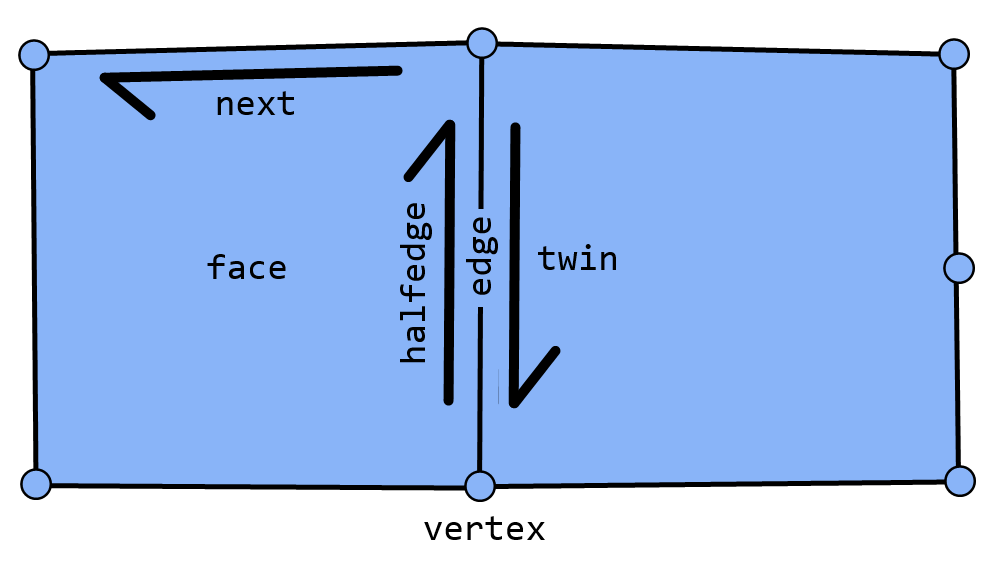
\includegraphics[width=0.55\textwidth]{HalfedgeMeshFigure_Quadrilateral}
		\caption{Halfedge meshes efficiently represent the connectivity information of a quadrilateral mesh, or any polyhedral mesh for that matter.
				Every vertex, full edge, and face has a pointer to a representative halfedge. Every halfedge has pointers to the face that contains them,
				the next halfedge around that face, the vertex it originated at, the full edge and face that it belongs to, and the twin halfedge on the other
				side of the halfedge's full edge. Extra information may be stored on each of these features, most notably the embedded  positions of each vertex in space.
				We could also store pointers to each halfedge's previous halfedge which is intuitively a reversal of the next pointers.}
		\label{fig:QuadrilateralHalfEdgeMesh}
		\end{figure}

		\paragraph{Orientation Definitions.}
		We would also like to take this opportunity to discuss some orientation details for transversing the mesh, e.g. while
		tracing a globally defined curve such as the silhouette curve that doesn't conform to any local patch coordinate system.
		We will define the \emph{edge number} $n(h)$ of a halfedge $h$ as follows:
		
		$$n(h) =
		\begin{cases}
		0 & \text{if $h = h \rightarrow \texttt{face} \rightarrow \texttt{half\_edge}$}\\
		n(h \rightarrow \texttt{prev}) + 1 & \text{otherwise.}
		\end{cases}$$

		We can use edge numbers to tell the relative orientation of neighboring patches. See Figure: \ref{fig:LocalCoordinateOrientations} for an illustration
		of all of the possible neighboring orientation relationships. Referring to the figure, if we want to transition from a point $(u, v)$ specified on the inner patch
		to one of the outer blue patches across an inner halfedge with edge number $n_{1}$ and an outer halfedge with edge number $n_{2}$
		we can do using Algorithm \ref{alg:Transition}. Note: if a tracing travels over a diagonal or travels more than a unitary distance in parameter space,
		we can simply apply the algorithm multiple times.

		\begin{figure}[h]
		\centering
		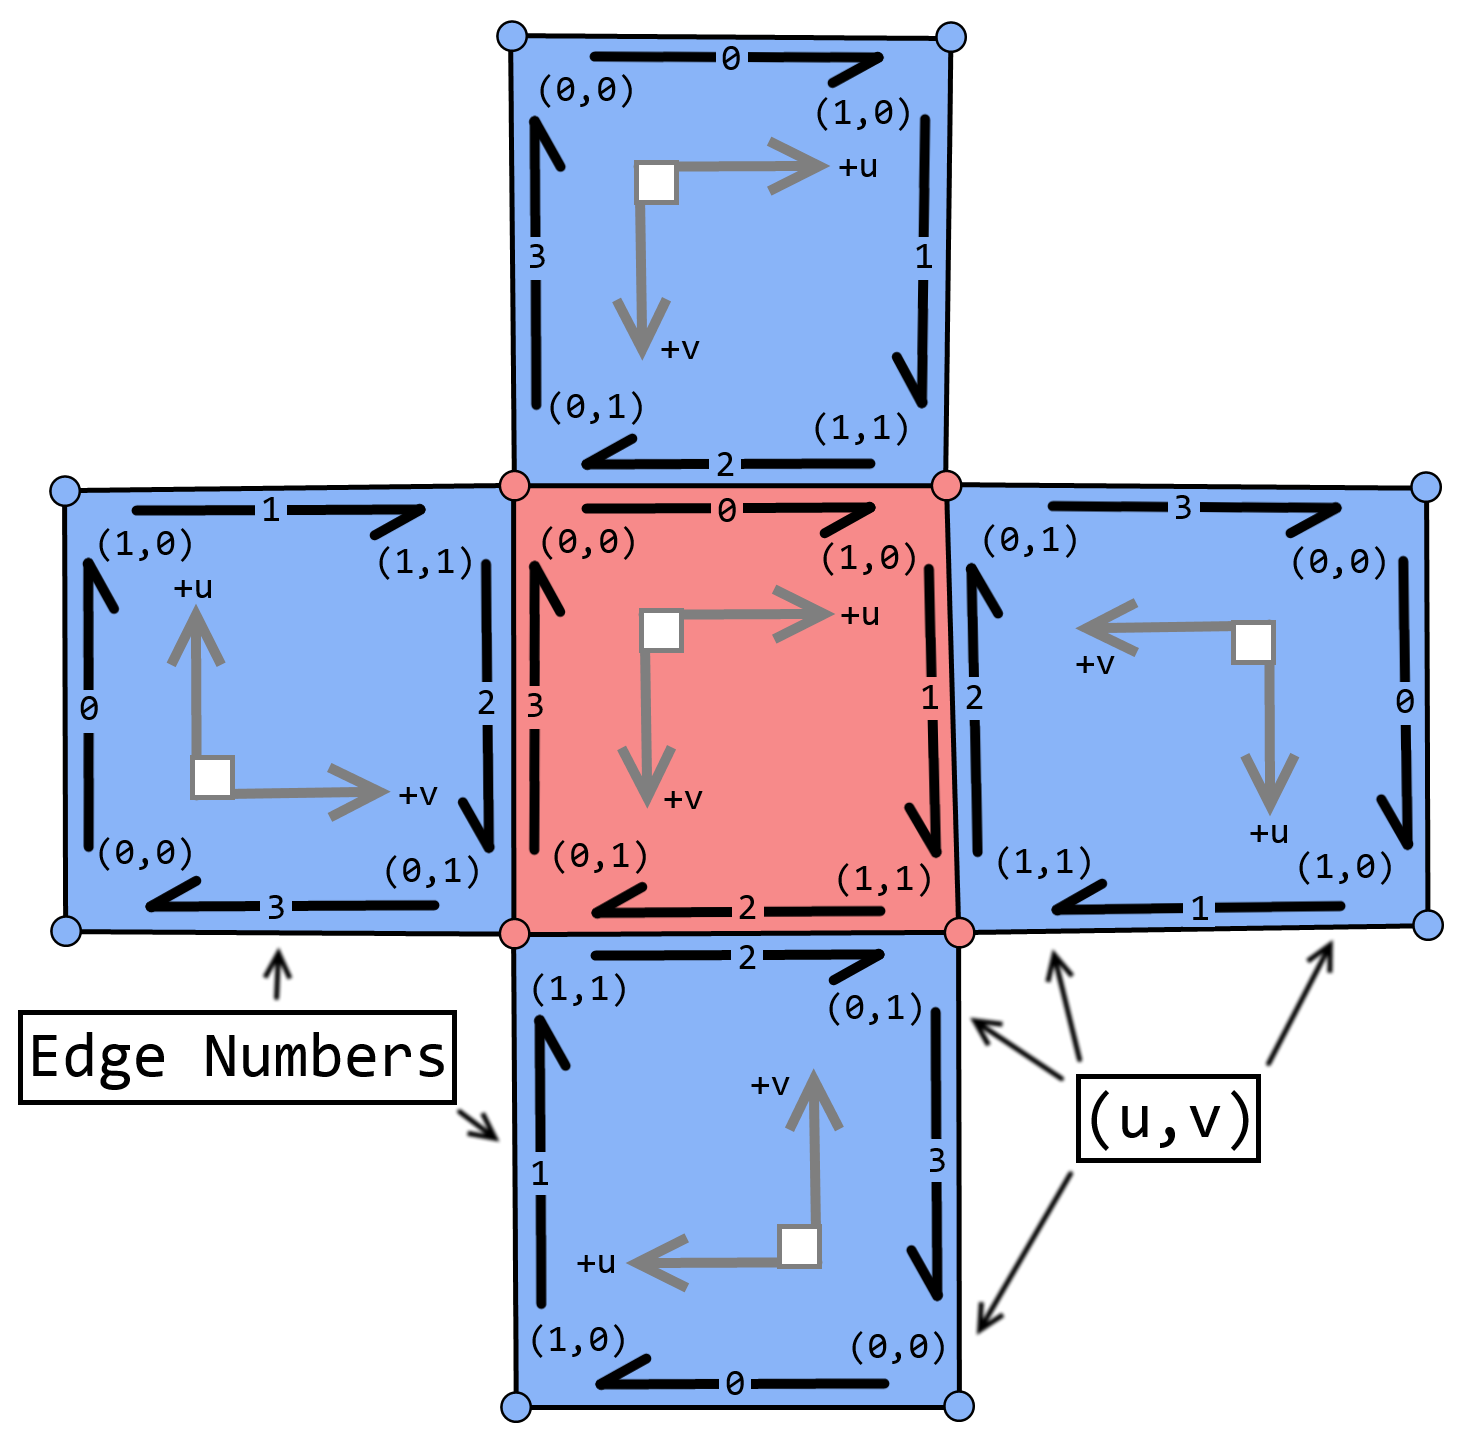
\includegraphics[width=0.75\textwidth]{LocalCoordinateTransversal}
		\caption{The four outer blue patches border the red inner patch in each for the four possible orientation relationships.
				Notice the arithmetic difference between the red patch edge numbers and its neighboring twin edge numbers is
				different for every possible orientation. Notice also that the local coordinate directions can flip after a transversal across a boundary.
				Because of this, it is important when designing algorithms to have them rely on global geometric properties, rather than local directions,
				such as the gradient along with a consistent handed choice of perpendicular direction.}
		\label{fig:LocalCoordinateOrientations}
		\end{figure}

		\begin{algorithm}                      % enter the algorithm environment
		\caption{Specifies a procedure for transitioning between local coordinate systems defined by a starting patch $p1$ and an ending patch $p2$ after travelling across a patch boundary.}
		\label{alg:Transition}       % and a label for \ref{} commands later in the document
		\begin{algorithmic}                    % enter the algorithmic environment
			\REQUIRE The surface must be represented via a halfedge mesh and utilize a consistent choice of local coordinate system based on the
					canonical halfedge for a given control mesh face.
			\ENSURE Properly transforms the input point from $p1$ to $p2$ within the unit rectangle parameter domain.
			\STATE \textbf{Start} at point $(u, v)$ in $p1$ space.
			\STATE $o1 \leftarrow$ edge number of $p1$.
			\STATE $o2 \leftarrow$ edge number of $p2$.
			\STATE $(u, v) \leftarrow (u, v) (mod 1)$ \COMMENT{Translation back into unit rectangle.}
			\STATE $n \leftarrow (o2 - o1 + 2)$ (mod 4). \COMMENT{Number of clockwise rotations.}
			\STATE $(u, v)  \leftarrow (u - .5, v - .5)$
			\FOR{$n$ times}
				\STATE $(u, v) \leftarrow (-v, u)$
			\ENDFOR
			\STATE $(u, v)  \leftarrow (u + .5, v + .5)$
			\STATE \textbf{end}
		\end{algorithmic}
		\end{algorithm}

	\newpage

	\subsection{Extracting Parameter Curves}

		Extracting parameter curves is quite straightforward. Start corner of a patch and then proceed in either the u or v direction as desired until you either get back to the original point or you encounter an extraordinary vertex.
		You may see a more formal description in Algorithm: \ref{alg:TraceParameterCurves}, noting that the computation is symmetric for the u or v direction.
		See Figure: \ref{fig:parameter_aligned_curves_torus} for an example of parameter curves extracted from a torus.

		\begin{algorithm}                      % enter the algorithm environment
		\caption{Given a surface, a point, and a fixed yet arbitrary u direction, this procedure computes the visible and nonvisible portions of an \textbf{axis aligned parameter curve}.}
		\label{alg:TraceParameterCurves}       % and a label for \ref{} commands later in the document
		\begin{algorithmic}                    % enter the algorithmic environment
			\REQUIRE The surface must be \textbf{continuous}, and parameterized via a quadrilateral control mesh.
			\ENSURE Returns a set of visible and nonvisible portions of the parameter curve going through the input point in the u direction.
			\STATE \textbf{begin}
				\STATE Start at point $G(u_{0}, v_{0})$
				\STATE $(u, v) \leftarrow (u_{0}, v_{0})$
			\REPEAT
				\STATE Start new curve.
				\IF{$f(u, v) < 0$}
				\STATE Mark curve as visible.
				\ELSE
				\STATE Mark curve as not visible.
				\ENDIF
				\STATE Add $g(u, v)$ with tangent $g_{u}(u, v)$ to curve.
				\REPEAT
				\STATE $u \leftarrow u + du$
				\STATE Add $G(u, v)$ with tangent $g_{u}(u, v)$ to curve.
				\IF{$u > 1$ or $u < 0$}
				\STATE Transition to a neighbor patch via Algorithm \ref{alg:Transition}.
				\STATE STOP if on a patch with an extraordinary vertex.
				\ENDIF
				\UNTIL{$f(u, v)$ changes sides.}
			\UNTIL{$(u, v) \approx (u_{0}, v_{0})$ on original patch within the step size.}
			\STATE \textbf{end}
		\end{algorithmic}
		\end{algorithm}

		\begin{figure}[h]
		\centering
		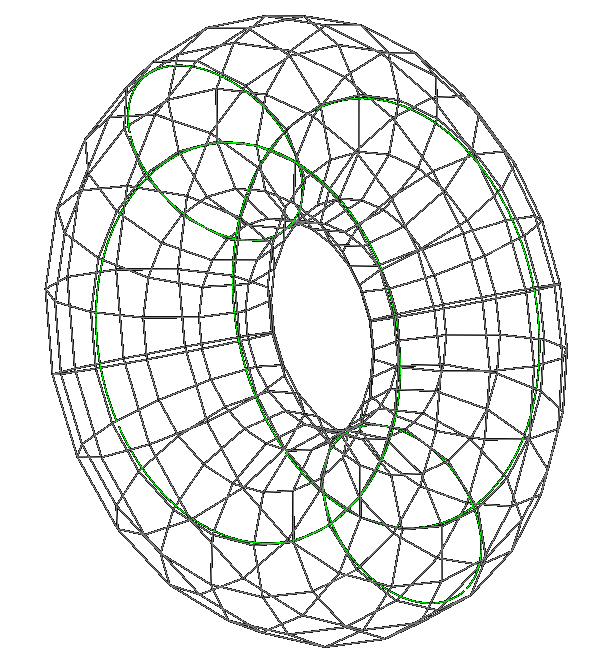
\includegraphics[width=0.5\textwidth]{Parameter_aligned_curves}
		\caption{Here are some example parameter curves along the two axis of a torus that were extracted by our system.
				Notice that the curves are smoother versions of the discrete lines constituting the control mesh.
				The control mesh was sculpted to follow the symmetries of the torus and therefore these parameter curves are
				useful in communicating the structure of the torus.}
		\label{fig:parameter_aligned_curves_torus}
		\end{figure}

	\newpage

	\subsection{Extracting the Morse-Smale Complex of a Scalar Function}
	\label{section:morse}
	
	In this section, we discuss the computation of a Morse-Smale Complex for an arbitrary scalar function $f$,
	which will allow us to extract unique representative points for every level set associated with a particular value in the range of $f$,
	such as silhouette curves, which are the 0 level set for the visibility function.

	\paragraph{Morse Functions.} A function $f(p)$ is \emph{Morse} if:

	\begin{itemize}
		\item $f$ is continuous and differentiable.
		\item All critical points are isolated.
		\item All critical points are non-degenerate, i.e. $\operatorname{det}(\operatorname{Hessian}(p))\ne 0$.
	\end{itemize}

	It is reasonable to assume that our functions will be \emph{Morse}, because our surfaces have $C_{1}$ continuity provided by the tangent patches,
	and most Catmull-Clark surfaces in general are not usually flat. If we needed to process flat surfaces, we could possibly perturb the input points to
	remove the analytic flatness, while retaining the visual flatness or we would process flat patches as special cases.

	\paragraph{Integral Lines.}

	An \emph{integral} curve $l$ is one that follows the gradient of a function $f$ from one critical point to another.
	In other words: $$\frac{\partial}{\partial t} = \nabla f(l(t)) \; \text{for all} \; t \in R$$ where R is the domain of $l$.

	\paragraph{Morse-Smale Complex.}
	The \emph{Morse-Smale Complex} of a function $f$ is an embedded graph on a surface formed by connecting every minima to every saddle point that it shares an 
	integral curve with and likewise connecting every maxima to each saddle point that it shares a curve with. This complex may be used to topologically segment
	the function. See Figure: \ref{fig:MorseSmale} an example.

	We can then use a Morse-Smale Complex computation as a means of extracting exactly one silhouette point from every unique silhouette curve that may
	be then used in our tracing algorithms. See Algorithm \ref{alg:findAllUniqueLevelSets}.


		\begin{algorithm}
		\caption{For a given height $h$, finds exactly 1 point on every level set defined for a function $f$ $\mathbb{R} \times \mathbb{R} \rightarrow \mathbb{R}$ on a surface $S$.}
		\label{alg:findAllUniqueLevelSets}
		\begin{algorithmic}

		\REQUIRE  $S$ has no boundary and is Morse.
		\ENSURE   Outputs a unique representative for every level set of height $h$.
		\STATE Initialize Morse-Smale complex graph $G$.
		\STATE Find all minima, maxima, and saddle points.
		\STATE Add critical points as vertices to $G$.
		\FOR{Every saddle point}
		\STATE Trace 2 integral curves up to 2 maxima.
		\STATE Trace 2 integral curves down to 2 minima.
		\STATE Add integral curves as edges to $G$.
		\IF{Curve crosses level $h$ during tracing}
			\STATE Remember the location on the edge.
		\ENDIF
		\ENDFOR

		\STATE \COMMENT {Union find algorithm separates $G$ into disjoint regions above and below the level sets.}
		\STATE Initialize a Union Find Structure $U$
		\STATE Make a set for vertex in $G$.
		\FOR{ $(c_{1}, c_{2}) \in Edges(G)$}
			\IF{$h \not \in [f(c_{1}, f(c_{2})]$}
				\STATE $U.\operatorname{union}(c_{1}, c_{2})$ \COMMENT{Union sets together if they are they do not cross the $h$ level.}
			\ENDIF
		\ENDFOR

		\FOR{ $e = (c_{1}, c_{2}) \in Edges(G)$}
			\IF{$U$.find($c_{1} \ne U.$find$c_{2}$}
				\STATE $U.\operatorname{union} (c_{1}, c_{2})$
				\STATE output the level set point location stored along $e$.
			\ENDIF
		\ENDFOR
		\end{algorithmic}
		\end{algorithm}


		\begin{figure}[h]
		\centering
		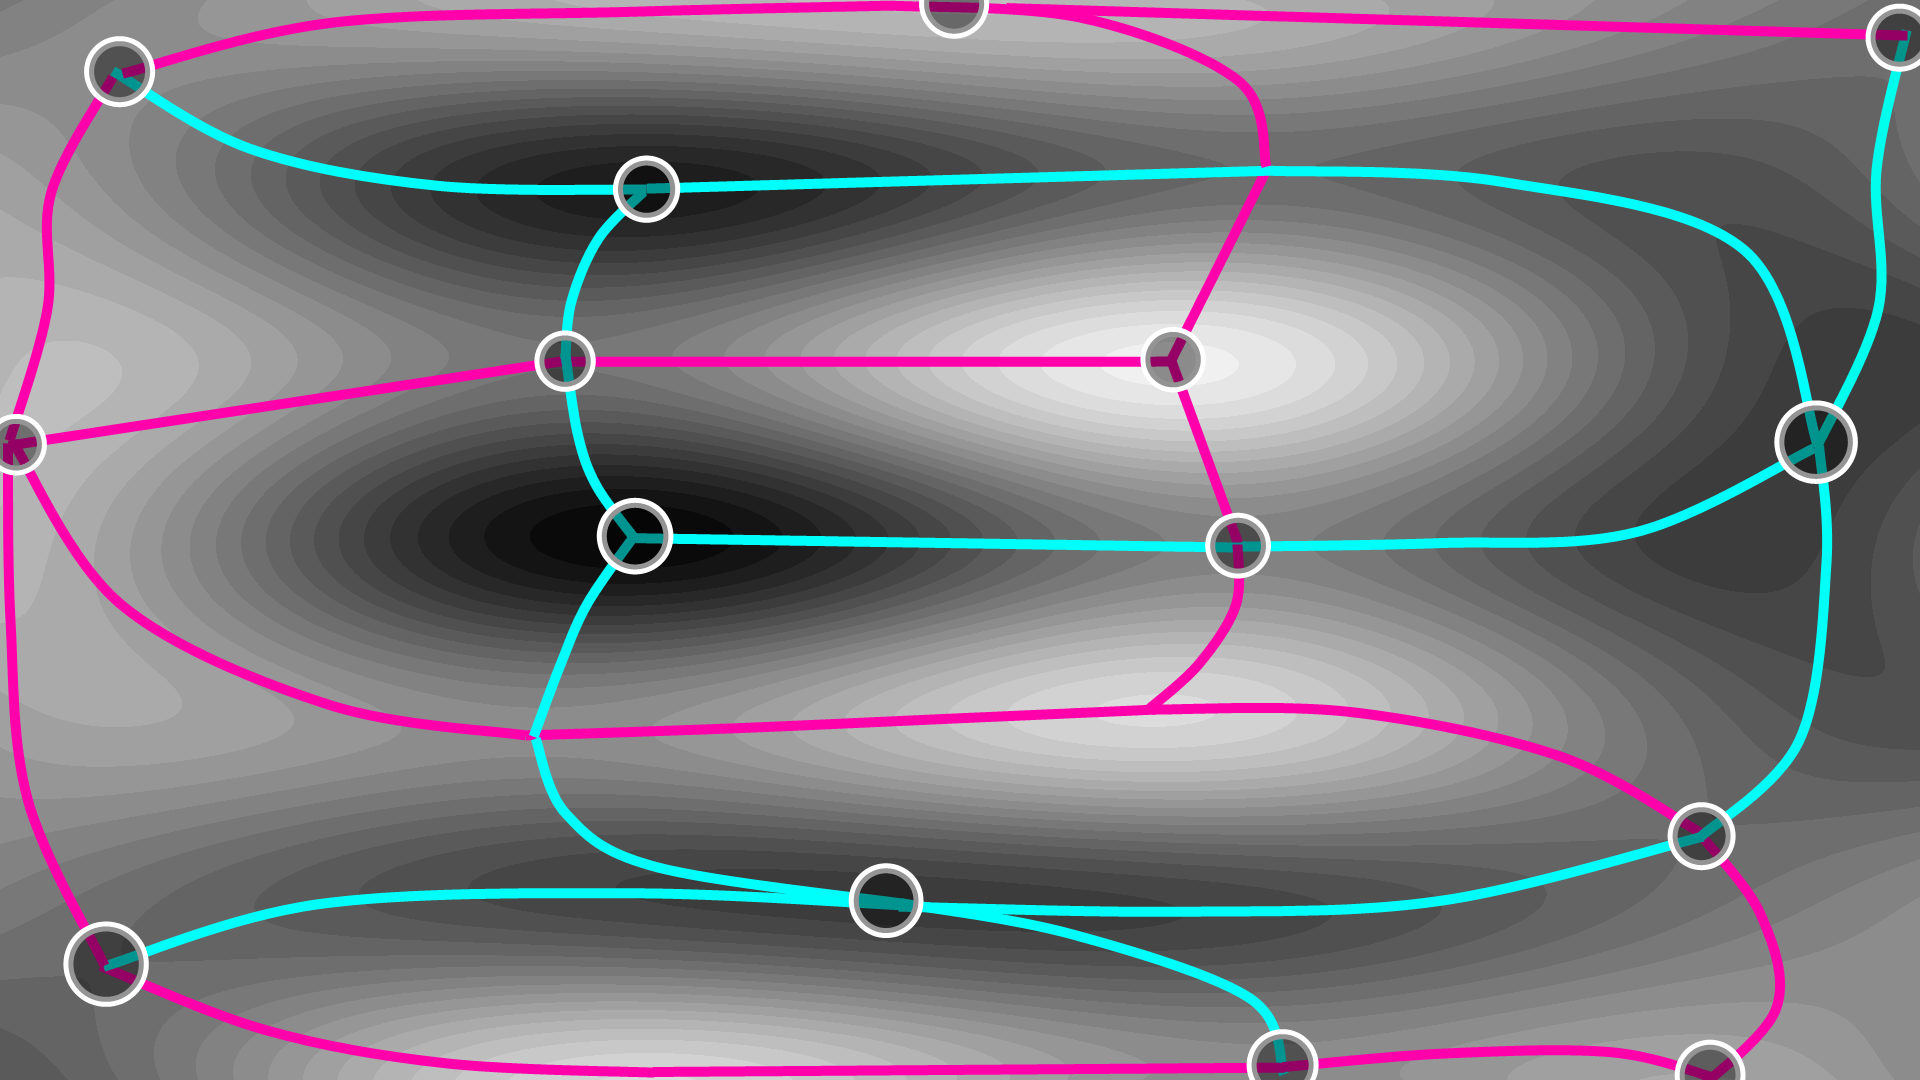
\includegraphics[width=0.5\textwidth]{minima_maxima_saddle_graph.png}
		\caption{Morse Smale Complex of the pullback of a function in two variables, i.e $\mathbb{R} \times \mathbb{R} \rightarrow \mathbb{R}$. Every saddle point connects to 2 minima and 2 maxima.}
		\label{fig:MorseSmale}
		\end{figure}


	\subsection{Extracting Silhouette Curves}

		\subsubsection{Finding Exact Representations of Silhouette Curves}
			We could potentially analytically extract all of the silhouette points on a surface by find the roots of multinomial equations defined by the visibility function,
			but that remains intractable at the present date and is an unsolved problem in the field of mathematics.
	
		\subsubsection{Curve Tracing Method}

			Because it is intractable to find the exact representations for silhouette curves, we use the practical curve tracing algorithm \ref{alg:TraceSilhouettes}.
			This algorithm is similar to the work of \cite{XJY98}.

			We find silhouette curves as follows:

			\begin{enumerate}
			\item Find all silhouette points that lie on patch boundaries. This may be accomplished via a 1D root finding algorithm in one parameter along the surfaces.
				Please see section \ref{section:findingSilhouettePoints} for more information.
			\item Trace the curves by starting at a silhouette point and repeatedly moving perpendicular to the gradient of the function,
				 then moving back to the silhouette curve by optimizing $$\nabla f^{2}(u, v)$$ When doing the optimization, use appropriate step bounding as in Section \ref{section:GD}.
			\end{enumerate}

			If the function is \emph{Morse}, we can alternatively find a unique collection of starting silhouette points via the Morse-Smale complex. Please see Section:
			\ref{section:morse}.

			%% Computes Silhouette Curves.
			\begin{algorithm}                      % enter the algorithm environment
			\caption{Given a surface, this algorithm computes a set of \textbf{silhouette curve discretizations},
				each consisting of silhouette points and corresponding tangent vectors pointing along the silhouette curve.
				We use an $\epsilon$ value of $.1$ which yields roughly $\frac{1}{\epsilon} = 10$ steps per patch, because each patch constitutes a 1 by 1 square in parameter space.} % give the algorithm a caption.
			\label{alg:TraceSilhouettes}       % and a label for \ref{} commands later in the document
			\begin{algorithmic}                    % enter the algorithmic environment
			    \REQUIRE The surface must be \textbf{continuous}, \textbf{differentiable}, and contain disjoint silhouette curves.
			    \ENSURE  If the surface has no boundaries, then the output curves are closed loops.
				\STATE \textbf{begin}
			    \STATE $S \Leftarrow $ Silhouette Point Finding Algorithm \ref{alg:FindSilhouettePoints}.
			    \FOR{Unvisited point $p \in S$}
				\STATE Mark $p$ as visited.
			        \STATE $(u_{0}, v_{0}) \leftarrow (p.u, p.v)$
				\STATE $(u, v) \leftarrow (u_{0}, v_{0})$
				\REPEAT
				        \STATE $(dv, -du) \leftarrow \nabla f(u,v)$
					\STATE normalize $(du, dv)$.
					\STATE $(u, v) \leftarrow (u, v) + \epsilon \cdot (du, dv)$
					\IF{$(u, v)$ out of unit rectangle bounds}
						\STATE Transition between patches via Algorithm \ref{alg:Transition}.
						\STATE mark boundary silhouette point as visited.
					\ENDIF
					\STATE $(u, v) \leftarrow $ GD $(\nabla(f^{2}),(u,v))$.
					\STATE Output point $g(u, v)$ and tangent $(du, dv)$.
				\UNTIL{$(u, v) \approx (u_{0}, v_{0})$ within the step size.}
			   \ENDFOR
				\STATE \textbf{end}
			\end{algorithmic}
			\end{algorithm}

			\begin{algorithm}                      % enter the algorithm environment.
			\caption{Given a surface, this algorithm finds the set of all silhouette points that lie on patch boundaries.} % give the algorithm a caption.
			\label{alg:FindSilhouettePoints}  % and a label for \ref{} commands later in the document.
			\begin{algorithmic}                    % enter the algorithmic environment.
			 	\REQUIRE The silhouette points on the boundaries need to be sufficiently far apart to prevent numerical instabilities.
				\ENSURE  
				\STATE \textbf{begin}
				\STATE $S \Leftarrow \emptyset$
				\FOR {$e \in Edges$}
					\STATE Compute the polynomial $p$ representing the silhouette function $f$ along $e$.
					\STATE Add all roots $\in [0, 1]$ of $p$ to $S$.
				\ENDFOR
			 	\STATE \textbf{return} $S$.
				\STATE \textbf{end}
			\end{algorithmic}
			\end{algorithm}

		\subsubsection{Finding Silhouette Points}
			\label{section:findingSilhouettePoints}

			Because it is intractable to find the exact representations for silhouette curves, we instead resort to finding a Silhouette points that 
			lie along the boundary of patches. Ideally we would like to only find one silhouette point per disjoint silhouette curve,
			which would eliminate the overhead of checking for curve equivalence,
			because otherwise we run the risk of tracing the same silhouette curves multiple times.
			If the function is \emph{Morse} we can accomplish this feat using the Morse-Smale Complex as in Section: \ref{section:morse}.



		\paragraph{1D Root Finding on Geometry Patches.}
		\label{section:rootFindingGeometryPatch}

		To find the silhouette points along a boundary of a geometry patch, we first expand the definition of the visibility function as follows:

		$$ f = E \cdot (G_{u} \times G_{v}) $$
		$$ G_{u}(u, v) = \sum_{i=0}^{3} \sum_{j=0}^{3} \mathcal{B'}_{i}^{3}(u) \mathcal{B}_{j}^{3} (v) G_{i, j} $$
		$$ G_{v}(u, v) = \sum_{i=0}^{3} \sum_{j=0}^{3} \mathcal{B}_{i}^{3}(u)  \mathcal{B'}_{j}^{3} (v) G_{i, j} $$

		If we assume that u = 0, then we can simplify these partial derivatives as follows:

		\begin{equation} \label{eq:Pv0v}
		P_{u} = -3 \sum_{j=0}^{3} \mathcal{B}_{j}^{3}(v) G_{0, j} + 3 \sum_{j=0}^{3} \mathcal{B}_{j}^{3}(v) G_{1, j}
		\end{equation}
		\begin{equation} \label{eq:Pu0v}
		P_{v} = \sum_{j=0}^{3} \mathcal{B'}_{j}^{3} (v) G_{0, j}
		\end{equation}

		To compute the silhouette points along a boundary or any other 1 - dimensional axis aligned slice of a patch, evaluate the partial derivative with either $u$ or $v$ set to a constant value,
		 such as $u = 0$ in Equations \ref{eq:Pv0v} and \ref{eq:Pu0v}. This results in partials represented by 3-dimensional vectors containing single variable polynomials for each dimension.
		The visibility function polynomial may then be computed directly form the visibility function formula applying the cross product and dot product operations as
		as normal, but with polynomial algebra, instead of scalar algebra. The resulting single variable polynomial represents the value of the visibility function 
		along the given axis aligned slice within the input variable domain [0, 1].
		The roots of this polynomial coorespond to Silhouette points. The roots may be computed using any single variable real root finding algorithm.
		We decided to implement root finding based on an interval bisection method using an interval counting method based on \emph{Sturm's theorem}\cite{AV10}, although numerical algorithms may have trouble discerning between roots that are sufficiently close to each other.
		They will also likely fail in the event of a silhouette curve runs along a boundary, because this will lead to an infinite number or roots.
		These Silhouette points work well, except when the silhouette curves cross boundaries between patches that contain extraordinary vertices.
		Please see Figure : \ref{fig:extraordinary_boundaries} for an example of the types of problematic behavior the extraordinary edges cause in our curve tracing algorithms.
		These problems provide the motivation for us to use tangent patches.

		\begin{figure}[h]
		\centering
		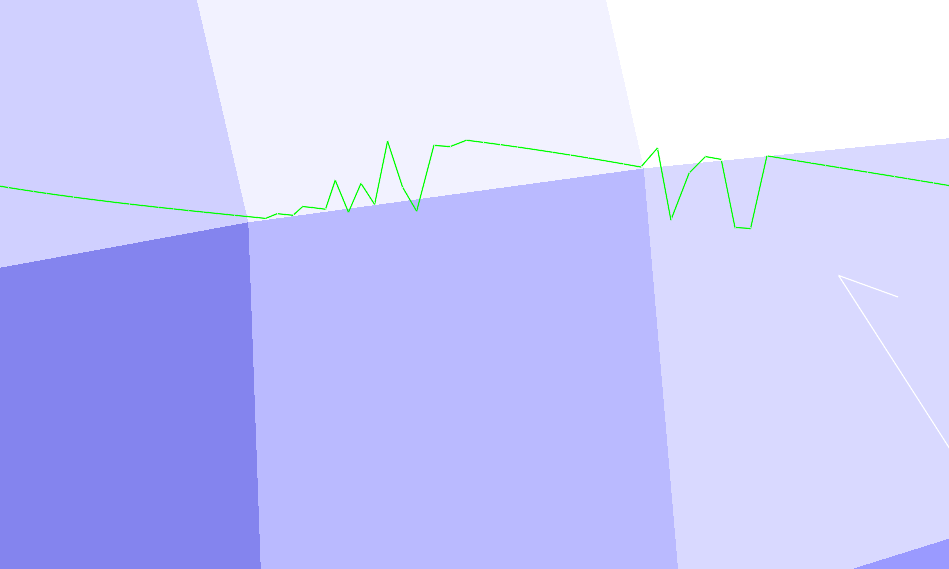
\includegraphics[width=0.5\textwidth]{ill_defined_silhouette_curves_over_extraordinary_boundary}
		\caption{Along extraordinary boundaries, the geometry patches are non-differentiable and therefore the visibility function is discontinuous. This causes curve tracing to fail due to an invalidation of its assumptions.}
		\label{fig:extraordinary_boundaries}
		\end{figure}

		\paragraph{1D Root Finding on Tangent Patches}

		To compute the roots of the tangent patch defined visibility curve, please use Equations \ref{eq:g_u} and \ref{eq:g_v} for the partials.
		Then apply the same parameter boundary substitution and again find the roots using polynomial vector algebra.

		\paragraph{Degenerate surface views.}

		Degenerate surface views occur whenever a surface is oriented such that its silhouette curves are not disjoint, such as viewing a torus in a manner perfectly orthogonal to its hole.
		Please see Figure : \ref{fig:degenerate_torus_orientation} for an example near degenerate view of a torus. They also occur for surface with flat patches.

		\begin{figure}[h]
		\centering
		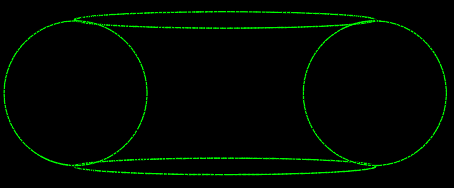
\includegraphics[width=0.5\textwidth]{torus_side_silhouettes}
		\caption{As a torus becomes oriented with its hole perpendicular to the viewing direction, its silhouette curves intersect each other. 
			This is one of several degenerate cases that present challenges to our curve tracing algorithms.}
		\label{fig:degenerate_torus_orientation}
		\end{figure}

		\subsubsection{Projecting 3D Discretizations onto 2D Planes}

		Curves may be projected onto 2D planes in several ways. The most rigorous way would be to convert
		the curves from their Bezier spline representations to rational splines directly. Another way would be to project their points
		using traditional perspective projection techniques used ubiquitous in rasterizers and project their tangents using the differential of the surface.
		So far, we are using a simple method, where we project the points using perspective projection and then project the points offset by their tangent direction
		to recover the tangent direction within the projection.


\section{Results}

We made a system that represents quadrilateral mesh defined Catmull-Clark subdivision surfaces through the Loop-Schaefer approximate via geometry and tangent patches.
We have developed some calculus for extracting curves on these surfaces, including the silhouette curves, parameter aligned curves, and integral curves in
We have developed algorithms for finding the location of critical points for the Silhouette function \textbf{F}
Please see Figure: \ref{fig:pig_silhouettes} to see some extracted silhouette curves from a pig model.
We have also been able to export SVG files containing our curves as paths. Please see Figure: \ref{fig:svg_export} for an example exported SVG file.
Please see the following URL for the latest research code we are using in our work: \url{https://github.com/Bryce-Summers/GeometricSurfaceCurves}.

\begin{figure}[h]
\centering
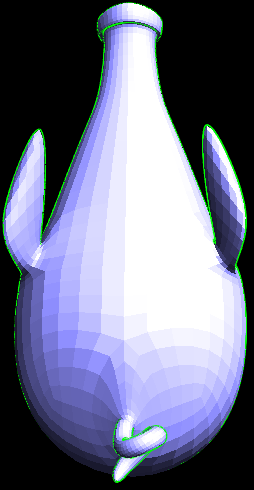
\includegraphics[width=0.25\textwidth]{Pig_patched}
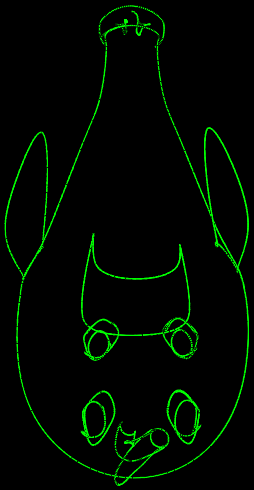
\includegraphics[width=0.25\textwidth]{Pig_silhouettes}
\caption{A view of a pig model rendered using Loop-Schaefer geometry patches and some silhouette curves extracted via our system.
	The green curves on the right represent silhouette curves that we have extracted from the view of the pig model on the left and include curves that are
	occluded from our view, such as those surrounding the pig's four feet. There are some kinks and instabilities in these curves that should theoretically
	disappear once we use tangent patches instead of geometry patches.}
\label{fig:pig_silhouettes}
\end{figure}

\begin{figure}[h]
\centering
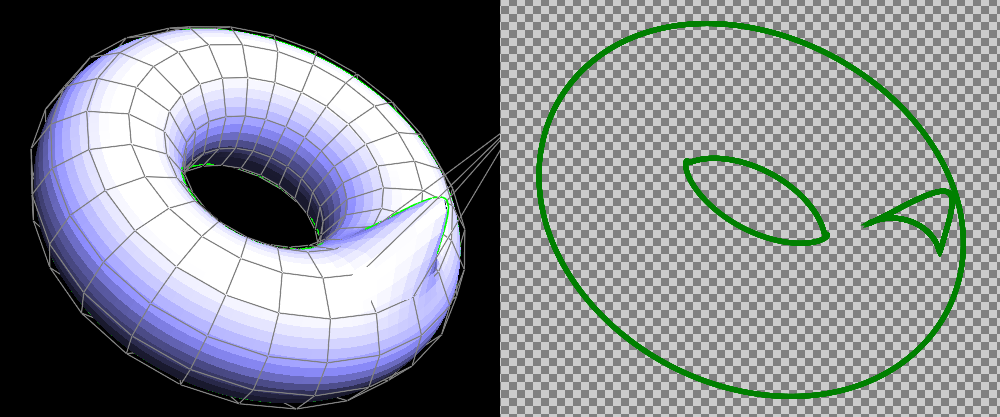
\includegraphics[width=0.5\textwidth]{SVG_Exportation}
\caption{A view of a modified toroidal surface with an associated exported SVG file.}
\label{fig:svg_export}
\end{figure}


\section{Comparison with prior work}

Past work including \cite{Eisemann08} has extracted silhouette curves from linear patches. They suffer from discontinuity and a lack of accurate interpolation of the points on the surface.
Please see Figure: \ref{fig:Eisemann_linear_patches} for an example of these problems. Please see Figure: \ref{fig:torus_silhouette_side_view} for an example silhouette curve that we extracted using our methods that is continuous everywhere and properly follows the surface.


\begin{figure}[h]
\centering
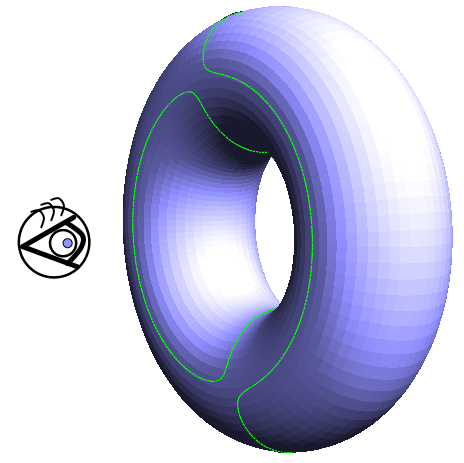
\includegraphics[width=0.5\textwidth]{torus_silhouettes_side_view}
\caption{Here are some silhouette curves extracted by our system that are continuous even when not viewed by their defining viewing direction.
		The green curves represent the silhouettes generated from a viewing of surface from the left as illustrated by the eyeball.}
\label{fig:torus_silhouette_side_view}
\end{figure}

\newpage

\section{Future Work}

Here we enumerate several problems that should be addressed in the future,
categorized into those that we feel can be immediately tackled, those that may need to wait for mathematics to progress a bit,
and those whose realization is tied to the development of artificial intelligence.

	\subsection{Near Term Problems}

	In this section we will describe several concisely stated problems similar to the silhouette curves problem that may be immediately tackled in the near future.

		\paragraph{Extracting the Exterior Silhouette Curve.}
		The actual visual exterior for a surface may include subsets of several silhouette curves. The exterior silhouette curve may be computed by projecting the
		non-occluded silhouette curves onto the view plane as a planar graph embedding and extracting the exterior face.		

		\paragraph{Shadows.}
		We can compute direct shadows	by computing the exterior silhouette curves from a light source viewing in the direction of the surface and then projecting this exterior silhouette 
		onto a plane representing the ground that the surface is resting on. Since our silhouette tracing algorithm may be used to trace an arbitrary
		scalar function, we could also potentially compute the shadows cast by an object onto an arbitrary curved surface by composing the 
		visibility function of the shadow casting surface with the projection onto another surface to extract complicated shadows or even self-shadows.

		\paragraph{Minimum and Maximum Curvature Curves.}
		Minimum and maximum curvature curves may be used to communicate information about geometrically intuitive local coordinate systems in the neighborhood of specific points on an object.
		It would be very useful to be able to derive a 2D coordinate grid given a point on a surface.
	
		\paragraph{Geodesic Curves.}
		In the future, a user should be able to specify two points on a surface and receive the curve that represents the minimum distance path between those two points.
		This is known as the curve of minimum geodesic distance.
	
		\paragraph{User Geometric Stylization Scheme.}
		Ideally, users could define a separation between geometric structure and the stylization applied to the geometry, much like cascading style sheets (CSS)
		define a separation between content and style in the display of web pages today. 
		Users would be able to convert entire presentations, including the technical figures and imagery from one style to another automatically.
		A user should be able to define their own figure color scheme, label placement policy, viewing lighting and shadow orientations, etc. in something like a CSS file and be able to automatically convert their figures between styles.

		\paragraph{Occlusion.}

		In our extracted curves, in addition to those points whose normals face away from the camera viewpoint,
		they may also include points that are not visible due to occlusion by other regions of the surface.
		There might be some interesting topological properties of closed curves that could be used for this task,
		especially if the homogenous depth of each of the points from the viewport was taken into account.

		\paragraph{Boundaries and Interiors}
		All of these problems could be extended to meshes with boundaries, which would also lead to the problem
		of properly handling communicating both the exterior and interior side of manifold surfaces with boundaries.
		It would also be interesting to think about handling the extraction of curves on non-orientable surfaces such as a M\"obius strip.

		\paragraph{Hot Wire Cutters.}

		Silhouette curves may be used to carve out surfaces without double negative curvature using hot wire cutters.
		There are some interesting problems related to this observation.

		\paragraph{Flat Patches}

		Flat patches cause many scalar function to be non-\emph{Morse}, because they lead to non-isolated critical points and large areas with 0 curvature.
		It will eventually be necessary to handle the problems associated with patches that contain 2D areas of silhouette points 
		due to them being oriented orthogonal to the viewpoint. These problem will also need to be dealt with if a future system wants to integrate
		Loop-Schaefer surfaces with traditional linear patch meshes.


	\subsection{Medium Term Problems}

		In this section, we describe several problems that are more difficult,
		mainly because they involve geometric computations of a higher degree than the current mathematics of our day can handle.
		
		\paragraph{Perspective Correct Silhouette Curves.}
		Right now, we are assuming that the user is viewing the surface with an orthonormal view perspective where the eye is looking in one uniform direction.
		This approximation leads to visually acceptable silhouette curve computations, but it is not accurate in terms of the actual perspective projection that the figures are rendered in.
		To compute the curves in a perspective correct manner would require higher degree geometric computations.

		\paragraph{Extracting Exact Geometric Curves.}
		Right now we are extracting points and tangents along curves, but if people were to solve the problem determining the root curves of multinomials, then we could represent these curves without discretization.
		This is a difficult problem in algebraic geometry that is connected to other seemingly hard problems in computer science.

		\paragraph{Labeling Geometry.}

		It would be interesting to develop algorithms for properly placing textual labels for a given figure view where the labels are aware of the geometry.
		The labels placing would have to take into account desirable properties, such as avoiding overlapping lines, avoiding intersections with other labels, and encouraging visual orientation coherence, whereby the labels would all face roughly the same way.
		Arrows could also be investigated.

		\paragraph{2D Segmenting and Labelling Ray Traced Imagery.}

		A system could hypothetically be built that segments a 2D projection of a ray traced scene into different regions based on light transport phenomena.
		Please see Figure \ref{fig:cornell_box_illustration}.

		\begin{figure}[h]
		\centering
		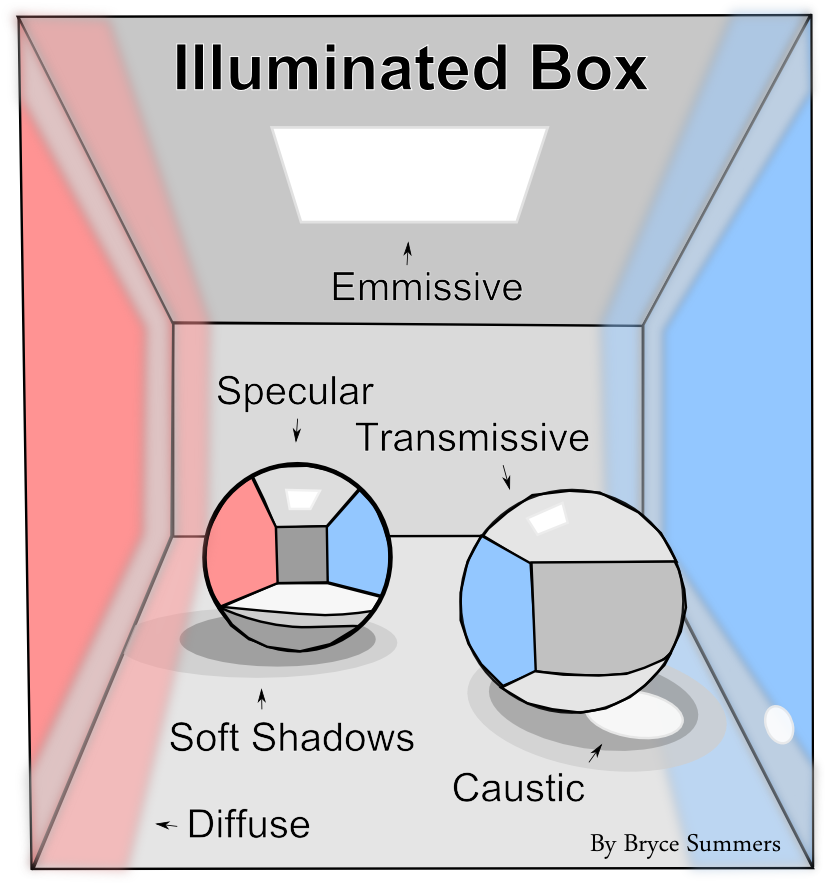
\includegraphics[width=0.5\textwidth]{cornell_box_illustration}
		\caption{A labeled illustration of the idea of converting a ray traceable scene into an SVG file with regions segmented by light transport phenomena.}
		\label{fig:cornell_box_illustration}
		\end{figure}


	\subsection{Long Term Problems}

		In this section, we will describe some long term grand problems that synthesize our work with Artificial Intelligence.

		\paragraph{Automatic Paper Interpreter.}
		In the future, a user could take a confusing research paper or any other work of communication feed it into a system and get a perfectly clear version of the paper back
		that even contains automatically generated illustrations of the ideas contained therein. This would enable us to reinterpret poorly written,
		poorly illustrated, or outdated papers in a form that is more readable and understandable for modern audiences and different types of learners.
		A person who shies away from mathematics or any other technical field because of the obtuseness of its academic literature would be able to 
		transform the writing into a more palatable form.

\newpage

\begin{thebibliography}{9}

\bibitem{JDA08}
Tilke Judd, Frédo Durand, and Edward Adelson. 2007. 
\emph{Apparent ridges for line drawing}. ACM Trans. Graph. 26, 3, Article 19 (July 2007). DOI=http://dx.doi.org/10.1145/1276377.1276401

Elmar Eisemann, Holger Winnemöller, John C. Hart, and David Salesin. 2008.
\emph{Stylized vector art from 3D models with region support}. In Proceedings of the Nineteenth Eurographics conference on Rendering (EGSR '08). Eurographics Association, Aire-la-Ville, Switzerland, Switzerland, 1199-1207. DOI=http://dx.doi.org/10.1111/j.1467-8659.2008.01258.x

\bibitem{Eisemann08}
Elmar Eisemann, Holger Winnemöller, John C. Hart, and David Salesin. 2008.
\emph{Stylized vector art from 3D models with region support}. In Proceedings of the Nineteenth Eurographics conference on Rendering (EGSR '08). Eurographics Association, Aire-la-Ville, Switzerland, Switzerland, 1199-1207. DOI=http://dx.doi.org/10.1111/j.1467-8659.2008.01258.x

\bibitem{Catmull98}
E. Catmull and J. Clark. 1998. \emph{Recursively generated B-spline surfaces on arbitrary topological meshes.}
In Seminal graphics. ACM, New York, NY, USA 183-188. DOI=http://dx.doi.org/10.1145/280811.280992

\bibitem{Stam98}
Jos Stam. 1998. 
\emph{Exact evaluation of Catmull-Clark subdivision surfaces at arbitrary parameter values.}
In Proceedings of the 25th annual conference on Computer graphics and interactive techniques (SIGGRAPH '98). ACM, New York, NY, USA, 395-404. DOI=http://dx.doi.org/10.1145/280814.280945

\bibitem{Loop}
Charles Loop and Scott Schaefer. 2008.
\emph{Approximating Catmull-Clark subdivision surfaces with bicubic patches}.
ACM Trans. Graph. 27, 1, Article 8 (March 2008), 11 pages. DOI=http://dx.doi.org/10.1145/1330511.1330519

\bibitem{XJY98}
Li Xuejun, Sun Jiaguang, and Yang Changgui. 1998.
\emph{Extracting Silhouette Curves of NURBS Surfaces by Tracing Silhouette Points}.
Tsinghua Science and Technology. ISSN 1007-0214, 13/22, pp1005 - 1008, Volume 3, Number 2. (June 1998), 4 pages.

\bibitem{SEH08}
Matei Stroila, Elmar Eisemann, and John Hart. 2008.
\emph{Clip Art Rendering of Smooth Isosurfaces}.
IEEE Transactions on Visualization and Computer Graphics 14, 1 (January 2008), 135-145. DOI=http://dx.doi.org/10.1109/TVCG.2007.1058

\bibitem{AV10}
Akritas, Alkiviadis G., and Panagiotis S. Vigklas. 2010.
\emph{Counting the Number of Real Roots in an Interval with Vincent's Theorem}.
Bulletin Mathématique De La Société Des Sciences Mathématiques De Roumanie 53 (101) (3). Societatea de Științe Matematice din România: 201–211. http://www.jstor.org/stable/43679177.

\bibitem{BS}
Jeffrey Bolz and Peter Schröder. 2002.
\emph{Rapid evaluation of Catmull-Clark subdivision surfaces.}
In Proceedings of the seventh international conference on 3D Web technology (Web3D '02). ACM, New York, NY, USA, 11-17. DOI=http://dx.doi.org/10.1145/504502.504505

\bibitem{Zorin06}
Denis Zorin. 2006.
\emph{Modeling with multiresolution subdivision surfaces.}
In ACM SIGGRAPH 2006 Courses (SIGGRAPH '06). ACM, New York, NY, USA, 30-50. DOI=http://dx.doi.org/10.1145/1185657.1185673

\bibitem{PXXZ15}
Qing Pan, Guoliang Xu, Gang Xu, and Yongjie Zhang. 2015.
\emph{Isogeometric analysis based on extended Loop's subdivision.}
J. Comput. Phys. 299, C (October 2015), 731-746. DOI=http://dx.doi.org/10.1016/j.jcp.2015.06.044

\bibitem{other}
http://www2.cs.uh.edu/~chengu/Teaching/Spring2013/Lecs/Lec8.pdf


\end{thebibliography}

\newpage

\section*{Appendix A: 3rd Order Bernstein Basis Functions and Derivatives}
\addcontentsline{toc}{section}{Appendix A: 3rd Order Bernstein Basis Functions and Derivatives.}

The Bernstein Basis functions of the third order are defined as follows:

$$B_{i} = \binom {3}{i} x^{i}(1 - x)^{3 - i}, \text{for} \; i \in \{0, \cdots, 3\}$$

Here is a listing of the four 3rd order Bernstein polynomials along with their 1st, and 2nd order derivatives:

\begin{align*}
B_{0} &= (1 - x)^{3} \; & B_{0}' &= -3(1-x)^{2} \; & B_{0}'' &= - 6x + 6\\
B_{1} &= 3x(1 - x)^{2} \; & B_{1}' &= (x - 1)(9x - 3) \; & B_{1}'' &= 18 x - 12\\
B_{2} &= 3x^{2}(1 - x) \; & B_{2}' &= (6 - 9x)x \; & B_{2}'' &= -18x + 6 \\
B_{3} &= x^{3} \; & B_{3}' &= 3x^{2} \; & B_{3}'' &= 6x\\
\end{align*}

Here is a listing of the 3rd order Bernstein polynomials in standard polynomial form along with their 1st derivatives in standard polynomial form:

\begin{align*}
B_{0} &= -x^{3} + 3x^{2} - 3x + 1 &B_{0}' &= -3x^{2} + 6x - 3\\
B_{1} &= 3x^{3} - 6x^{2} + 3x      &B_{1}' &= 9x^{2} - 12x + 3\\
B_{2} &= -3x^{3} + 3x^{2} &B_{2}' &= 9x^{2} + 6x\\
B_{3} &= x^{3} &B_{3}' &= 3x^{2}\\
\end{align*}

%%// FIXME: Consider putting a lovely picture here illustrating the Bernstein Polynomials.

\newpage

\section*{Appendix B: 2nd Order Bernstein Basis Functions and Derivatives}
\addcontentsline{toc}{section}{Appendix B: 2nd Order Bernstein Basis Functions and Derivatives}

The Bernstein Basis functions of the third order are defined as follows:

$$B_{i} = \binom {2}{i} x^{i}(1 - x)^{2 - i}, \text{for} \; i \in \{0, \cdots, 2\}$$

Here is a listing of the 2nd order Bernstein polynomials along with their 1st, and 2nd order derivatives:

\begin{align*}
B_{0} &= (1 - x)^{2} \;& B_{0}' &= 2x - 2 \; & B_{0}'' &= 2\\
B_{1} &= 2x(1-x) \;& B_{1}' &= -4x + 2 \; & B_{1}'' &= -4\\
B_{2} &= x^{2} \;& B_{2}' &= 2x \; & B_{2} &= 2\\
\end{align*}


Here is a listing of the three 2nd order Bernstein polynomials in standard polynomial form along with their 1st derivatives in standard polynomial form:

\begin{align*}
B_{0} &= x^{2} - 2x + 1 \; & B_{0}' &= 2x - 2 \; & B_{0}'' &= 2\\
B_{1} &= -2x^{2} + 2x \; & B_{1}' &= -4x + 2 \; &B_{1}'' &= -4\\
B_{2} &= x^{2} \; & B_{2}' &= 2x \; &B_{2}'' &= 2\\
\end{align*}

%%// FIXME: Consider putting a lovely picture here illustrating the Bernstein Polynomials.

\newpage

%% Here is where I am putting a bunch of the large figures, which might inhibit the flow of the paper when they are placed inline.

\end{document}